\documentclass[a4paper,fleqn]{article}

% title and author
\title{Process Algebra and mCRL2\\
\emph{\large IPA Basic Course on Formal Methods 2006}\\
{\normalsize 19th January 2006}}
\author{Jan Friso Groote \and Aad Mathijssen \and Bas Ploeger \and Michel
Reniers \and Muck van Weerdenburg \and Jeroen van der Wulp} 
\date{}

% packages
\usepackage{pstricks,pst-node,pstcol,pst-grad,pst-plot,pst-coil}
\usepackage[english]{babel}
\usepackage[final]{graphics}
\usepackage{amsmath}
\usepackage{amsfonts}
\usepackage{array}
\usepackage{calc}
\usepackage{xspace}
\usepackage{color}
\usepackage{epsfig}
\usepackage{subfigure}
\usepackage{stmaryrd}
\usepackage{times}
\usepackage{float}
\usepackage{fancyhdr}

% General layout
% --------------

% increase pagewidth
\addtolength{\textwidth}{20mm}
\addtolength{\oddsidemargin}{-10mm}
\addtolength{\evensidemargin}{10mm}

%add headings
\pagestyle{fancy}
\fancyhead{}
\renewcommand{\headrulewidth}{0pt}

% set the indentation of the math environment to 10mm
\setlength{\mathindent}{10mm}

% equations are unique up to their section
\renewcommand{\theequation}{\arabic{equation}}

% do not put subsubsections in the table of contents
\addtocounter{tocdepth}{-1}

% column types that change column types l,c,r from math mode to LR
% and the other way round
\newcolumntype{L}{>{$}l<{$}}%stopzone%stopzone%stopzone
\newcolumntype{C}{>{$}c<{$}}%stopzone%stopzone%stopzone
\newcolumntype{R}{>{$}r<{$}}%stopzone%stopzone%stopzone

% Environments
% ------------

% equations: eqnarray environment with no outer column spacing and tighter
% intercolumn spacing
\newenvironment{equations}
  {\setlength{\arraycolsep}{2pt}%
   \begin{array}{@{}lll@{}}%
  }
  {\end{array}%
  }

% tightarray: array with no outcolumn spacing and tighter intercolumn spacing
\newenvironment{tightarray}[1]
  {\setlength{\arraycolsep}{2pt}%
   \begin{array}{@{}#1@{}}%
  }
  {\end{array}%
  }

% definitions: list of definitions where:
% - the optional argument denotes the space between successive items
%   (default 0.15em)
% - items are horizontally aligned at the math indent
\newenvironment{definitions}[1][0.15em]
  {\begin{list}%
    {}%
    {\setlength{\parsep}{0pt}%
     \setlength{\itemsep}{#1}%
     \setlength{\leftmargin}{\mathindent}%
     \setlength{\labelwidth}{\mathindent - \labelsep}%
    }
  }
  {\end{list}}

% tdefinitions: list of tagged definitions where:
% - the optional argument denotes the space between successive items
%   (default 0.15em)
% - items are horizontally aligned at the math indent
% - each item is tagged with the mandatory argument
\newenvironment{tdefinitions}[2][0.15em]
  {\begin{list}%
    {#2}%
    {\setlength{\parsep}{0pt}%
     \setlength{\itemsep}{#1}%
     \setlength{\leftmargin}{\mathindent}%
     \setlength{\labelwidth}{\mathindent - \labelsep}%
    }
  }
  {\end{list}}

% edefinitions: list of enumerated definitions where:
% - the optional argument denotes the space between successive items
%   (default 0.15em);
% - items are horizontally aligned at the math indent;
% - each item is numbered with a parenthesised roman numeral.
\newcounter{edefinitioncount}
\newenvironment{edefinitions}[1][0.15em]
  {\begin{list}%
    {(\roman{edefinitioncount})}%
    {\renewcommand{\theenumi}{\roman{enumi}}%
     \renewcommand{\labelenumi}{(\theenumi)}%
     \usecounter{edefinitioncount}%
     \setlength{\parsep}{0pt}%
     \setlength{\itemsep}{#1}%
     \setlength{\leftmargin}{\mathindent}%
     \setlength{\labelwidth}{\mathindent - \labelsep}%
    }
  }
  {\end{list}}
  
% entry: list of entries where:
% - the optional argument denotes the space between successive items
%   (default 0.15em);
% - items are horizontally aligned at the math indent;
% - each item is labelled.
\newenvironment{entry}[2][0.15em]%
  {\begin{list}{}%
    {\renewcommand{\makelabel}[1]{\textsf{##1:}\hfil}%
     \settowidth{\labelwidth}{\textsf{#2:}}%
     \setlength{\leftmargin}{\labelwidth+\labelsep}%     
     \setlength{\parsep}{0pt}%
     \setlength{\itemsep}{#1}%
    }%
  }%
  {\end{list}}

% derivation: calculational derivation where expressions (\expr) are related by
% means of transformations (\tran). A transformation is denoted by a symbol and
% a hint. Expressions and transformations can be broken into several lines
% using \breakexpr and \breaktran.
\newenvironment{derivation}
{\par\addtolength{\baselineskip}{1mm}\begin{tabbing}\hspace{5mm}\=\hspace{5mm}\=\hspace{5mm}\=\kill}
{\end{tabbing}\par}
\newcommand{\expr}[1]{\>\>$#1$}
\newcommand{\tran}[2]{\\*\>$#1$\>\>\{ #2 \}\\}
\newcommand{\trannoassert}[1]{\\*\>$#1$\>\>\\}
\newcommand{\breakexpr}{$\\*\>\>$}
\newcommand{\breaktran}{\\*\>\>\>\hspace{8pt}}

% Theorem-like environments that are numbered as s.n, where:
% - s is the section number
% - n is the number of occurrences of all theorem-like environments in s
% We have the following environments:
% - definition
% - theorem
% - lemma
% - corollary
% - property
% - example
% - remark
% - convention
% - specification
% - declaration

\newtheorem{thdefinition}{Definition}[section]
\newenvironment{definition}
  {\begin{thdefinition}\em}
  {\end{thdefinition}}

\newtheorem{ththeorem}[thdefinition]{Theorem}
\newenvironment{theorem}
  {\begin{ththeorem}\em}
  {\end{ththeorem}}

\newtheorem{thcorollary}[thdefinition]{Corollary}
\newenvironment{corollary}
  {\begin{thcorollary}\em}
  {\end{thcorollary}}

\newtheorem{thlemma}[thdefinition]{Lemma}
\newenvironment{lemma}
  {\begin{thlemma}\em}
  {\end{thlemma}}

\newtheorem{thproperty}[thdefinition]{Property}
\newenvironment{property}
  {\begin{thproperty}\em}
  {\end{thproperty}}

\newtheorem{thexample}[thdefinition]{Example}
\newenvironment{example}
  {\begin{thexample}\em}
  {\end{thexample}}

\newtheorem{thremark}[thdefinition]{Remark}
\newenvironment{remark}
  {\begin{thremark}\em}
  {\end{thremark}}

\newtheorem{thconvention}[thdefinition]{Convention}
\newenvironment{convention}
  {\begin{thconvention}\em}
  {\end{thconvention}}

\newtheorem{thspecification}[thdefinition]{Specification}
\newenvironment{specification}
  {\begin{thspecification}\em}
  {\end{thspecification}}

\newtheorem{thdeclaration}[thdefinition]{Declaration}
\newenvironment{declaration}
  {\begin{thdeclaration}\em}
  {\end{thdeclaration}}

\newtheorem{thexercise}[thdefinition]{Exercise}
\newenvironment{exercise}
  {\begin{thexercise}\em}
  {\end{thexercise}}

% proof: proof of a theorem
\newenvironment{proof}
  {\textbf{Proof}}
  {\frm{\Box}
   \vspace{1ex}%
  }


% Commands
% --------
% --------


% math mode
% ---------

% improvement to $ ... $ such that mathematical formulas cannot be cramped
\newcommand{\frm}[1]{\mbox{\ensuremath{#1}}}

% frm with extra spacing
\newcommand{\for}[1]{\frm{\,#1\,}}


% functions and constants
% -----------------------

% constant
\newcommand{\f}[1]{\ensuremath{\mathit{#1}}}

% function application with 1 argument: f(arg0)
\newcommand{\fa}[2]{\ensuremath{\f{#1}(#2)}}

% function application with 2 arguments: f(arg0, arg1)
\newcommand{\faa}[3]{\ensuremath{\f{#1}(#2, #3)}}

% function application with 3 arguments: f(arg0, arg1, arg2)
\newcommand{\faaa}[4]{\ensuremath{\f{#1}(#2, #3, #4)}}

% function application with 4 arguments: f(arg0, arg1, arg2, arg3)
\newcommand{\faaaa}[5]{\ensuremath{\f{#1}(#2, #3, #4, #5)}}


% functions and types
% -------------------

% function application symbol: .
\newcommand{\fap}{\ensuremath{\!\cdot\!}}

% composition: 0
\newcommand{\comp}{\ensuremath{\circ}}

% function composition: o
\newcommand{\fcomp}{\ensuremath{%
  \hspace{0.08em}\mbox{\small\ensuremath{\circ}}\hspace{0.08em}}}
  
% function mapping
\newcommand{\fmap}{
  \hspace{0.08em}\raisebox{0.2ex}{%
  \tiny\ensuremath{\bullet}}\hspace{0.08em}}


% lambda calculus
% ---------------

% abstraction in the typed lambda calculus
\newcommand{\labst}[3]{\ensuremath{\lambda #1\!:\!#2.#3}}

% application in the typed lambda calculus
\newcommand{\lappl}[2]{\ensuremath{#1\ #2}}

% abstraction in the pure (untyped) lambda calculus
\newcommand{\pabst}[2]{\ensuremath{\lambda #1.#2}}

% application in the pure (untyped) lambda calculus
\newcommand{\pappl}[2]{\ensuremath{#1\ #2}}

% sets
% ----

% set of elements: {e}
\newcommand{\set}[1]{\ensuremath{\{\,#1\,\}}}

% bag of elements: {e}
\newcommand{\bag}[1]{\ensuremath{\set{#1}}}

% set difference: s \ t
\newcommand{\sdiff}[2]{\ensuremath{#1\ \backslash\ #2}}

% set comprehension: { e | c }, where e is an expression or a binding and c is
% a condition
\newcommand{\scompr}[2]{\ensuremath{\set{#1\ |\ #2}}}

% powerset: P(s)
\newcommand{\pow}[1]{\ensuremath{\fa{\mathcal{P}}{#1}}}


% tuples
% ------

% tuple of elements: <e>
\newcommand{\tpl}[1]{\ensuremath{\langle\,#1\,\rangle}}

% pair of elements: <e0,e1>
\newcommand{\pair}[2]{\ensuremath{\tpl{#1\hspace{0.08em},#2}}}


% lists
% -----

% list of a certain type: L(t)
\newcommand{\List}[1]{\ensuremath{\mathcal{L}{\I{#1}}}}

% list of elements: [e]
\newcommand{\lst}[1]{\ensuremath{[\,#1\,]}}

% empty list
\newcommand{\el}{\ensuremath{[\,]}}

% cons: |>
\newcommand{\cons}{\ensuremath{\hspace{0.12em}\triangleright\hspace{0.08em}}}
  
% snoc: <|
\newcommand{\snoc}{\ensuremath{\hspace{0.08em}\triangleleft\hspace{0.12em}}}

% concatenation: ++
\newcommand{\concat}{\ensuremath{\hspace{0.12em}\raisebox{0.2ex}
{\text{\footnotesize+}\!\text{\footnotesize+}}\hspace{0.12em}}}

% take
\newcommand{\take}{\ensuremath{\lceil}}

% drop
\newcommand{\drop}{\ensuremath{\lfloor}}


% logic
% -----

% boolean type: B
\newcommand{\bool}{\ensuremath{\mathbb{B}}}

% true
\newcommand{\true}{\ensuremath{\f{true}}}

% false
\newcommand{\false}{\ensuremath{\f{false}}}

% implies: =>
\newcommand{\limp}{\ensuremath{\Rightarrow}}

% follows: =>
\newcommand{\lfol}{\ensuremath{\Leftarrow}}

% bi-implies: <=>
\newcommand{\lbimp}{\ensuremath{\Leftrightarrow}}

% not with extra spacing
\newcommand{\Lnot}{\ensuremath{\ \lnot\ }}

% and with extra spacing
\newcommand{\Land}{\ensuremath{\ \land\ }}

% or with extra spacing
\newcommand{\Lor}{\ensuremath{\ \lor\ }}

% implies with extra spacing
\newcommand{\Limp}{\ensuremath{\ \limp\ }}

% bi-implies with extra spacing
\newcommand{\Lbimp}{\ensuremath{\ \lbimp\ }}

% quantification in Dijkstra notation: <Q x : y : z>
\newcommand{\quantD}[4]{\ensuremath{\langle\,{#1} {#2} : #3 : {#4}\,\rangle}}

% universal quantification in Dijkstra notation: <forall x : y : z>
\newcommand{\forallD}[3]{\ensuremath{\quantD{\forall}{#1}{#2}{#3}}}

% existential quantification in Dijkstra notation: <exists x : y : z>
\newcommand{\existsD}[3]{\ensuremath{\quantD{\exists}{#1}{#2}{#3}}}

% derivable in #1: |-_#1
\newcommand{\derivable}[1]{\ensuremath{\vdash_{_{#1}}}}

% valid in #1: |=_#1
\newcommand{\valid}[1]{\ensuremath{\models_{_{#1}}}}

%inference rule with 0 premises and 1 conclusion
\newcommand{\infC}[1]{\ensuremath{
  \begin{array}{c} 
    \\\hline 
    #1 
  \end{array}
}}

%inference rule with 1 premise and 1 conclusion
\newcommand{\infPC}[2]{\ensuremath{
  \begin{array}{c} 
    #1 \\\hline 
    #2 
  \end{array}
}}

% inference rule with 2 premises and 1 conclusion
\newcommand{\infPPC}[3]{\ensuremath{
  \begin{array}{c@{\hspace{2em}}c}
    #1 & #2 \\\hline
    \multicolumn{2}{c}{#3}
  \end{array}
}}

%inference rule with 3 premises and 1 conclusion
\newcommand{\infPPPC}[4]{\ensuremath{
  \begin{array}{c@{\hspace{2em}}c@{\hspace{2em}}c}
    #1 & #2 & #3\\\hline
    \multicolumn{3}{c}{#4}
  \end{array}
}}

% arithmetic
% ----------

% natural type: N
\newcommand{\nat}{\ensuremath{\mathbb{N}}}

% positive type: P
\newcommand{\pos}{\ensuremath{\nat^{+}}}

% integral type: Z
\newcommand{\tint}{\ensuremath{\mathbb{Z}}}

% non-negative real type: R^{>=0}
\newcommand{\nnreal}{\ensuremath{\mathbb{R}^{\geq 0}}}

% integer division: "div"
\renewcommand{\div}{\ensuremath{\ \mathbf{div}\ }}

% integer remainder: "mod"
\renewcommand{\mod}{\ensuremath{\ \mathbf{mod}\ }}


% miscellaneous
% -------------

% first uses of a term go in this font
\newcommand{\deffont}[1]{\textbf{#1}}

% language of a signature Sigma: L(Sigma)
\newcommand{\lang}[1]{\ensuremath{\fa{\mathcal{L}}{\f{#1}}}}

% meaning of a syntactic element
\newcommand{\mean}[1]{%
  [\hspace{-.15em}[\hspace{.15em}#1\hspace{.15em}]\hspace{-.15em}]%
}

% sequential composition .
\newcommand{\seq}{\mathbin{\cdot}}

% alternative composition +
\newcommand{\alt}{\mathbin{+}}

% parallel merge ||
\newcommand{\pmerge}{\mathbin{\parallel}}

% left merge ||_
\newcommand{\lmerge}{\mathbin{\llfloor}}

% synchronisation |
\newcommand{\sync}{\mathbin{\!\mid\!}}

% block
\newcommand{\block}[1]{\partial_{#1}}

% hide
\newcommand{\hide}[1]{\tau_{#1}}

% rename
\newcommand{\ren}[1]{\rho_{#1}}

% allow
\newcommand{\allow}[1]{\nabla_{#1}}

% communication
\newcommand{\comm}[1]{\Gamma_{#1}}

% at
\font \aap cmmi10        
\newcommand{\at}[1]{\mbox{\aap ,} #1}

% ???
\newcommand{\ap}{{:}}

% compatibility definitions for axioms
\def\ax{=}
\def\axle{\le}
\def\bm#1{#1_\delta}
\newcommand{\mb}[1]{\text{\boldmath$#1$}}% Simple bold math
\def\toset#1{#1_{\{\}}}
\def\tobag#1{#1_{\langle\rangle}}
\def\tomact#1{#1_{\mid}}
\def\bag#1{\langle #1 \rangle}

% bullet
\newcommand{\bul}{\mbox{\small\ensuremath{\bullet}}}

% complexity according to expression: O(e)
\newcommand{\bigo}[1]{\ensuremath{\mathcal{O}(#1)}}

% print #2 inside #3, where #2 is raised by #1
\newlength{\insidewd}%                        Define length command
\newcommand{\inside}[3][0pt]{%		      Definition of inside:
   \settowidth{\insidewd}{#3}%                - Save width of #3
   \raisebox{#1}[0pt]{%                       - Raise #2 by #1
     \makebox[0pt]{\hspace{\insidewd}#2}}%    - Print #2 centered
   #3}%				              - Print #3

% stack #2 on #3, where #2 is raised by #1
\newlength{\stackht}%                         Define length commands
\newcommand{\stack}[3][0pt]{%		      Definition of stack:
   \settoheight{\stackht}{#3}%                - Save height of #3
   \addtolength{\stackht}{#1}%                - Add to #1 to height
   \inside[\stackht]{#2}{#3}}%                - Print #2 in #3 at height #3 + #1

% abbreviations
% -------------

% mCRL
\newcommand{\mCRL}{\frm{\mu}CRL\xspace}

% Miscellaneous local definitions
% -------------------------------

% temporary lengths
\newlength{\tlength}

% mCRL2 keywords
\newcommand{\kwsort}{{\bf sort}}
\newcommand{\kwcons}{{\bf cons}}
\newcommand{\kwmap}{{\bf map}}
\newcommand{\kwvar}{{\bf var}}
\newcommand{\kweqn}{{\bf eqn}}
\newcommand{\kwact}{{\bf act}}
\newcommand{\kwstruct}{{\bf struct}}
\newcommand{\kwwhr}{{\bf whr}}
\newcommand{\kwend}{{\bf end}}
\newcommand{\kwdiv}{{\bf div}}
\newcommand{\kwmod}{{\bf mod}}
\newcommand{\kwproc}{{\bf proc}}
\newcommand{\kwinit}{{\bf init}}


% mCRL2 Sorts
\newcommand{\srtbool}{\f{Bool}}
\newcommand{\srtpos}{\f{Pos}}
\newcommand{\srtnat}{\f{Nat}}
\newcommand{\srtint}{\f{Int}}
\newcommand{\srtreal}{\f{Real}}

\newenvironment{mcrl2}%
{\par\bigskip\noindent%
 \begin{tabular}{@{}>{\bf}p{2.3em}L@{\ }L@{\ }L@{\ }L@{\ }L@{\ }L@{\ }L@{\ }L}%
}%
{\end{tabular}\bigskip\par%
}

\begin{document}

\maketitle

\section{Introduction}
\label{sec:introduction}

In a typical distributed system, a number of components are running
simultaneously in parallel. By working together, these components provide the
functionalities that are required from the complete system. Although the
behaviour of a single component can usually be specified and analysed relatively
easily, the behaviour of the system as a whole is often too complex to be
specified or analysed thoroughly. This is primarily due to (and inherent to) the
parallelism between the system's components. An exhaustive analysis of all of
the system's states and execution paths thus becomes a formidable task -- even
for a system with a relatively small number of components.

In this part of the IPA Basic Course on Formal Methods, we introduce and explain
process algebra, which is a formalism that is well suited for the specification
of system behaviour. This is done within the context of the mCRL2 specification
language \cite{Groote et al 2005} and toolset \cite{mCRL2 toolset}. With the
toolset, users can specify the behaviour of a distributed system and analyse it
using automated techniques. In Section \ref{subsec:history} we give a short
history of mCRL2. In Section \ref{subsec:overview} we give an overview of the
remainder of this document.

\subsection{History}
\label{subsec:history}

As its name suggests, mCRL2 is the successor of the \mCRL specification language
and toolset \cite{Groote 1997, Groote Ponse 1994, Groote Reniers 2001}. The
\mCRL toolset has been developed at and maintained by the Centre for Mathematics
and Computer Science (CWI) in Amsterdam since the beginning of the nineties of
the previous century. The \mCRL language extends a basic process algebra --
based on the Algebra of Communicating Processes (ACP) \cite{Baeten Weijland
1990} -- with the possibility to define and use abstract data types.  The
ability to use data within a process algebra specification is a valuable
(perhaps even a necessary) enhancement when applying the toolset to a real-life
system.

The \mCRL language has clear and well-defined syntax and semantics. Over the
years, various tools have been developed for \mCRL, all with a strong foundation
in formal theories. The toolset has been used in numerous case studies for the
analysis of systems and protocols developed by both the industry and the
academic world (see for example \cite{Fokkink et al 2004, Groote et al 2003,
Pang et al 2003}). In nearly all cases the analysis revealed errors in the
system being analysed.

Recently, researchers at the Eindhoven University of Technology (TU/e) started
the development of the mCRL2 language and toolset. Based on user experiences
with \mCRL, their focus is to develop a more user friendly language and tool
interface. The most substantial improvement to the language on the data side is
the introduction of predefined and higher-order data types, lambda calculus
expressions and various other language constructs that are designed to make the
data type definitions shorter and easier to read and write. Regarding the
process algebra, the most remarkable change is the introduction of multiactions
which allow for a more straightforward conversion of Petri nets to mCRL2
specifications. Furthermore, the language is truly compositional, meaning that
large systems can be specified in terms of smaller components. Finally, the
mCRL2 toolset is being extended with a graphical user interface which improves
the usability of the toolset and can be used alongside the traditional command
line interface.

\subsection{Overview}
\label{subsec:overview}

\begin{figure}[tbp]
\centering
  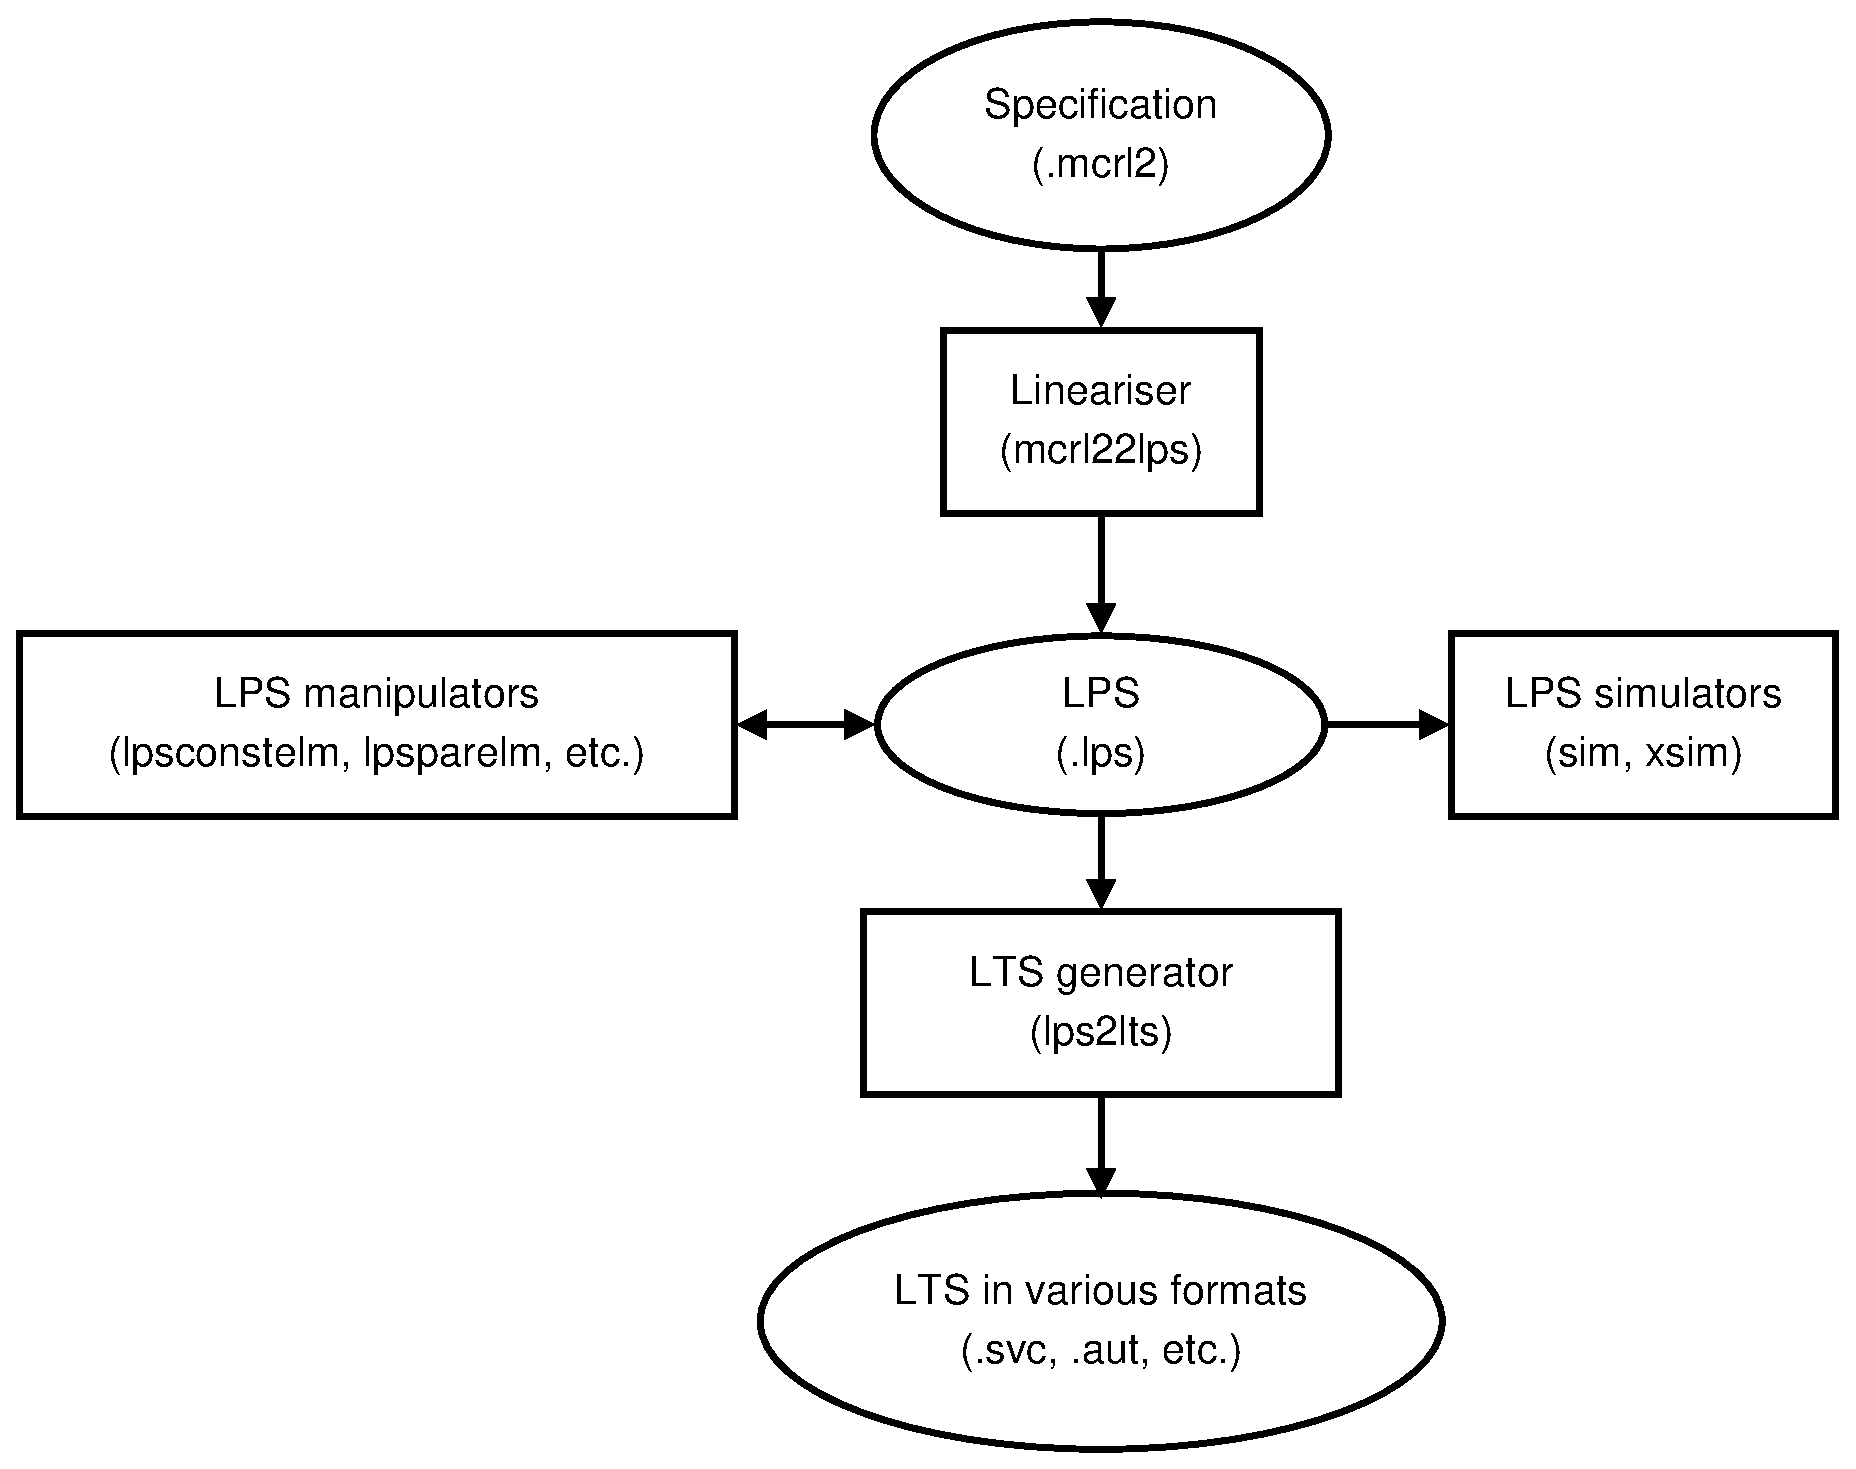
\includegraphics[scale=0.4]{mcrl2_toolset}
  \caption{Overview of the mCRL2 toolset}
  \label{fig:overview}
\end{figure}

In general, the following steps are involved in the analysis of a system with
mCRL2 (see also Figure~\ref{fig:overview}):
\begin{itemize}
  \item A specification of the system's behaviour is written in the mCRL2
    language.
  \item This specification is converted to a \emph{Linear Process Equation}
    (LPE) by the mCRL2 lineariser tool. As we shall see, an LPE is an
    mCRL2 specification in a stricter format.
  \item The LPE can be modified using various manipulation tools and can be
    simulated using various simulation tools.
  \item A \emph{Labelled Transition System} (LTS) or \emph{state space} is
    generated from the modified LPE.
\end{itemize}

\noindent Subsequently, this LTS can be analysed for errors using model
checking techniques. This is a topic which is beyond the scope of this
document. The remainder of this document contains the following sections:
\begin{itemize}
  \item Language (Section \ref{sec:language});
  \item Linear Process Equations (Section \ref{sec:lpe});
  \item Toolset (Section \ref{sec:toolset}).
\end{itemize}

\noindent Every section contains exercises to practise the material during the
course. 

\section{Language}
\label{sec:language}

This section describes the mCRL2 language. Roughly, the language consists of
a process algebra part and data specification part. These parts are explained
in Sections \ref{ssec:process algebra} and \ref{ssec:data}, respectively.

The precise syntax of the language can be found in Appendix \ref{sec:syntax}.
Note that this syntax, which is used in this and the following sections, uses a
rich text format. The toolset, however, uses a plain text format, which is
related to the rich notation in Appendix \ref{sec:symbols}.

\subsection{Process algebra}
\label{ssec:process algebra}

The most basic notion in the mCRL2 process language is an \deffont{action}.
Actions represent atomic events. The following example illustrates how actions
$\f{send}$, $\f{receive}$ and $\f{error}$ can be declared:
\begin{mcrl2}
act & send, receive;\\
    & error;
\end{mcrl2}

\noindent
In general we write $a,b,\ldots$ to denote actions.

\deffont{Process expressions}, denoted by $p,q,\ldots$, describe when certain
actions can be executed. For example, ``$a$ is followed by either $b$ or $c$''. We
make this notion more formal by introducing operators.

\subsubsection{Basic operators}
\label{ssec:basic operators}

\noindent
Process expressions are compositions of actions using a number of operators.
The most basic expressions are as follows:
\begin{itemize}
\item \deffont{Actions} $a$, $b$ etc. as described above.

\item \deffont{Deadlock} or inaction $\delta$, which does not display any
behaviour.

\item \deffont{Alternative composition}, written as $p \alt q$. This
represents a \emph{non-deterministic choice} between $p$ and $q$.

\item \deffont{Sequential composition}, written $p \seq q$. This expression
first executes $p$ and then $q$ (assuming $p$ terminates).
\end{itemize}

\noindent
When writing process expressions we usually omit parentheses as much as
possible. To do this, we give $\seq$ a higher precedence than $\alt$ and use
the associativy of both operators. So, instead of writing $(a\seq (b\seq
c))\alt(d\alt e)$ we usually write $a\seq b\seq c\alt d\alt e$.

To give meaning to processes we use LTSs. In Figure~\ref{fig.lts.example} the
LTS corresponding to the process expression $a\seq b\alt c\seq(d\seq\delta\alt
e)$ is shown. To be able to distinguish deadlock ($\delta$) and successful
termination (e.g. after an action $a$) we use closed nodes to indicate that a
process has terminated and open nodes if a process has not (yet) done so. Each
open node, usually called a state, corresponds to a process described by the
(sub-)graph with this node as root. In Figure~\ref{fig.lts.example} we have
labelled the states with the corresponding process expressions.

\begin{figure}[H]
\centering
\begin{pspicture}(3,4)
\psset{arrows=->,arrowsize=6pt,radius=.2}
 \Cnode(1,4){0}
 \Cnode(0,2){1}
 \Cnode[fillstyle=solid,fillcolor=black](0,0){2}
 \Cnode(2,2){3}
 \Cnode(1,0){4}
 \Cnode[fillstyle=solid,fillcolor=black](3,0){5}
 \nput{0}{0}{\textcolor{gray}{$a\seq b\alt c\seq(d\seq\delta\alt e)$}}
 \nput{0}{1}{\textcolor{gray}{$b$}}
 \nput{0}{3}{\textcolor{gray}{$d\seq\delta\alt e$}}
 \nput{0}{4}{\textcolor{gray}{$\delta$}}
 \ncline{0}{1}\tlput{a}
 \ncline{1}{2}\tlput{b}
 \ncline{0}{3}\trput{c}
 \ncline{3}{4}\tlput{d}
 \ncline{3}{5}\trput{e}
\end{pspicture}
\caption{LTS of $a\seq b\alt c\seq(d\seq\delta\alt e)$}
\label{fig.lts.example}
\end{figure}

In Figure~\ref{fig.lts} the LTSs for the basic operators are drawn.
Figure~\ref{fig.lts.p} denotes the LTS for a general process, meaning that
$p_0$ is the (only) initial state of $p$ and $p_1$ to $p_n$ ($n\ge 0$) are its
terminating states. As shown in Figure~\ref{fig.lts.alt}, the alternative
composition of two processes is created by merging their initial states. For
the sequential composition $p\seq q$ each of the terminating states of $p$ is
replaced with a copy of $q$ (Figure~\ref{fig.lts.seq}).

\begin{figure}[H]
\centering
\mbox{
\subfigure[$\delta$]{
\begin{pspicture}(2,2.5)
\psset{arrows=->,arrowsize=6pt,radius=.2}
 \Cnode(1,1.5){0}
\end{pspicture}
\label{fig.lts.delta}
}\hspace{4em}
\subfigure[$a$]{
\begin{pspicture}(2,2.5)
\psset{arrows=->,arrowsize=6pt,radius=.2}
 \Cnode(1,2.5){0}
 \Cnode[fillstyle=solid,fillcolor=black](1,0.5){1}
 \ncline{0}{1}\trput{$a$}
\end{pspicture}
\label{fig.lts.a}
}\hspace{4em}
\subfigure[$p$]{
\begin{pspicture}(2,2.5)
\psset{arrows=->,arrowsize=6pt,radius=.2}
 \Cnode(1,2.5){0}
 \Cnode[fillstyle=solid,fillcolor=black](0,0.5){1}
 \Cnode[fillstyle=solid,fillcolor=black](2,0.5){2}
 \nput{0}{0}{$p_0$}
 \nput{180}{1}{$p_1$}
 \nput{0}{2}{$p_n$}
 \ncline[arrowsize=0,linestyle=dashed]{0}{1}%\tlput{$a_1$}
 \ncline[arrowsize=0,linestyle=dashed]{0}{2}%\trput{$a_n$}
 \ncline[arrowsize=0,linestyle=dotted]{1}{2}
\end{pspicture}
\label{fig.lts.p}
}\hspace{4em}
}\\\vspace{1em}
\mbox{
\subfigure[$p\alt q$]{
\begin{pspicture}(4,5)
\psset{arrows=->,arrowsize=6pt,radius=.2}
 \Cnode(2,4){0}
 \Cnode[fillstyle=solid,fillcolor=black](0,2.8){1}
 \Cnode[fillstyle=solid,fillcolor=black](0.5,2){2}
 \Cnode[fillstyle=solid,fillcolor=black](3.5,2){3}
 \Cnode[fillstyle=solid,fillcolor=black](4,2.8){4}
 \nput{0}{0}{$p_0,q_0$}
 \nput{180}{1}{$p_1$}
 \nput{0}{2}{$p_n$}
 \nput{180}{3}{$q_1$}
 \nput{0}{4}{$q_m$}
 \ncline[arrowsize=0,linestyle=dashed]{0}{1}%\tlput{$a_1$}
 \ncline[arrowsize=0,linestyle=dashed]{0}{2}%\trput{$a_n$}
 \ncline[arrowsize=0,linestyle=dashed]{0}{3}%\tlput{$b_1$}
 \ncline[arrowsize=0,linestyle=dashed]{0}{4}%\trput{$b_m$}
 \ncline[arrowsize=0,linestyle=dotted]{1}{2}
 \ncline[arrowsize=0,linestyle=dotted]{3}{4}
\end{pspicture}
\label{fig.lts.alt}
}\hspace{4em}
\subfigure[$p\seq q$]{
\begin{pspicture}(5,5)
\psset{arrows=->,arrowsize=6pt,radius=.2}
 \Cnode(2.5,5){0}
 \Cnode(1,3){1}
 \Cnode(4,3){2}
 \Cnode[fillstyle=solid,fillcolor=black](0,1){3}
 \Cnode[fillstyle=solid,fillcolor=black](2,1){4}
 \Cnode[fillstyle=solid,fillcolor=black](3,1){5}
 \Cnode[fillstyle=solid,fillcolor=black](5,1){6}
 \nput{0}{0}{$p_0$}
 \nput{180}{1}{$p_1,q_0$}
 \nput{0}{2}{$p_n,q_0$}
 \nput{270}{3}{$q_1$}
 \nput{270}{4}{$q_m$}
 \nput{270}{5}{$q_1$}
 \nput{270}{6}{$q_m$}
 \ncline[arrowsize=0,linestyle=dashed]{0}{1}%\tlput{$a_1$}
 \ncline[arrowsize=0,linestyle=dashed]{0}{2}%\trput{$a_n$}
 \ncline[arrowsize=0,linestyle=dotted]{1}{2}
 \ncline[arrowsize=0,linestyle=dashed]{1}{3}%\tlput{$b_1$}
 \ncline[arrowsize=0,linestyle=dashed]{1}{4}%\trput{$b_m$}
 \ncline[arrowsize=0,linestyle=dotted]{3}{4}
 \ncline[arrowsize=0,linestyle=dashed]{2}{5}%\tlput{$b_1$}
 \ncline[arrowsize=0,linestyle=dashed]{2}{6}%\trput{$b_m$}
 \ncline[arrowsize=0,linestyle=dotted]{5}{6}
 \psdots(2,2)(2.5,2)(3,2)
\end{pspicture}
\label{fig.lts.seq}
}
}
\caption{LTSs of the basic operators}
\label{fig.lts}
\end{figure}

\begin{exercise}\label{exc.lts}
Draw the LTS for each of the following processes:
\begin{enumerate}
\item $(a\alt b)\seq c$ \label{exc.lts.1}
\item $a\seq c\alt b\seq c$ \label{exc.lts.2}
\item $a\alt\delta$
\item $\delta\seq(a\alt b)$
\end{enumerate}
\end{exercise}

\noindent
Looking at Exercises \ref{exc.lts}.\ref{exc.lts.1} and
\ref{exc.lts}.\ref{exc.lts.2}, we see that after doing either an $a$ or a $b$
both processes have exactly the same behaviour (namely $c$). To express this
equality with respect to the (observable) behaviour a process describes we use
\deffont{(strong) bisimulation equivalence}. Which processes are equal, or
\emph{bisimilar}, according to this equivalence is stated as follows. For every
action one process can perform, the other has to be able to perform the same
action as well \emph{and} the resulting processes should be bisimilar.
Furthermore, if one process has terminated the other should have done so as
well. For example, $a\seq(b\alt c)$ can perform an $a$, which results in a
process $b\alt c$, and $a\seq b\alt a\seq c$ can also perform an action $a$,
but not such that the resulting process is equal to $b\alt c$. Thus, these
processes are not {\it bisimilar}.

Other equivalences can also be used. With \deffont{trace equivalence}, for
instance, two processes are equal when the sets of traces that the processes
can execute are equal.\footnote{We will not define the set of traces of a
process formally.} In this case $a\seq(b\alt c)$ and $a \seq b\alt a \seq c$,
which are not bisimilar, would be equivalent as for both we have that
$\{\epsilon,a,a\seq b,a\seq c\}$, with $\epsilon$ the empty trace, is the set
of traces.

We explain our choice for bisimilarity by means of the story ``The Lady, or the
Tiger?'' by Frank Stockton \cite{Stockton}, which tells about a barbaric king
who puts his accused subjects in the middle of a public arena. In this arena,
there are two closed doors, exactly alike. The fate, and thereby also the
guilt, of the accused is decided by forcing him to open one of the two.  Behind
one of the doors is a hungry tiger which will tear him to pieces immediately
when given the opportunity. The other conceals a beautiful lady to whom, once
revealed, he will be married instantly.

When modelling such a trial, we treat the opening of the doors as an atomic
action, as well as the resulting behaviour after opening each of the doors. The
correct model for the above story is $\f{open\_door}\seq\f{marry\_lady} \alt
\f{open\_door}\seq\f{confront\_tiger}$, as depicted in
Figure~\ref{fig.lady_or_tiger.good}. It expresses that whether you will be
confronted with the lady or the tiger depends on the $\f{open\_door}$ action.
The model $\f{open\_door}\seq(\f{marry\_lady}\alt\f{confront\_tiger})$ in
Figure~\ref{fig.lady_or_tiger.bad}, however, is wrong, because after opening a
door the accused person can somehow still choose between meeting the tiger and
marrying the lady.

\begin{figure}[H]
\centering
\mbox{
\subfigure[]{
\begin{pspicture}(2,4)
\psset{arrows=->,arrowsize=6pt,radius=.2}
 \Cnode(1,4){0}
 \Cnode(0,2){1}
 \Cnode(2,2){2}
 \Cnode[fillstyle=solid,fillcolor=black](0,0){3}
 \Cnode[fillstyle=solid,fillcolor=black](2,0){4}
 \ncline{0}{1}\tlput{$\f{open\_door}$}
 \ncline{0}{2}\trput{$\f{open\_door}$}
 \ncline{1}{3}\tlput{$\f{marry\_lady}$}
 \ncline{2}{4}\trput{$\f{confront\_tiger}$}
\end{pspicture}
\label{fig.lady_or_tiger.good}
}\hspace{14em}
\subfigure[]{
\begin{pspicture}(2,4)
\psset{arrows=->,arrowsize=6pt,radius=.2}
 \Cnode(1,4){0}
 \Cnode(1,2){1}
 \Cnode[fillstyle=solid,fillcolor=black](0,0){2}
 \Cnode[fillstyle=solid,fillcolor=black](2,0){3}
 \ncline{0}{1}\trput{$\f{open\_door}$}
 \ncline{1}{2}\tlput{$\f{marry\_lady}$}
 \ncline{1}{3}\trput{$\f{confront\_tiger}$}
\end{pspicture}
\label{fig.lady_or_tiger.bad}
}
}
\caption{The lady, or the tiger?}
\label{fig.lady_or_tiger}
\end{figure}

\noindent
We use \deffont{axioms} to express the properties of the operators.  The axioms
for the operators introduced so far are listed in Table \ref{ax.basic}. Here,
$x,y,z$ are variables that stand for unknown process expressions. With the
axioms we can prove, for instance, $a\alt(\delta\alt a)$ equal to $a$ using
axioms A2, A6 and A3 as follows:
\begin{center}
$a\alt(\delta\alt a)\;\stackrel{\mathrm{A2}}{=}\;(a\alt\delta)\alt
a\;\stackrel{\mathrm{A6}}{=}\;a\alt a\;\stackrel{\mathrm{A3}}{=}\;a$
\end{center}


\begin{table}[htbp]
\begin{center}
\fbox{\begin{tabular}{lL}
A1 & x\alt y\ax y\alt x  \\
A2 & x\alt (y\alt z)\ax(x\alt y)\alt z  \\
A3 & x\alt x\ax x  \\
A4 & (x\alt y) \seq z\ax x \seq z\alt y \seq z  \\
A5 & (x \seq y) \seq z\ax x \seq (y \seq z)  \\
A6 & x\alt \delta\ax x  \\
A7 & \delta \seq x\ax\delta  \\
\end{tabular}}
\caption{Basic operator axioms}
\label{ax.basic}
\end{center}
\end{table}

\noindent
We introduce more axioms along the way. In Appendix \ref{sec:axioms} a complete
overview of all axioms is given. Note that some axioms given in this section
are slightly simplified versions of those given in Appendix \ref{sec:axioms}
due to the incremental structure of this document.

\begin{exercise}\label{exc.basic}
Prove the following propositions:
\begin{enumerate}
\item $a\alt(\delta\alt a)\;\ax\;a$ (without using axiom A2) 
\item $\delta\seq(a\alt b)\;\ax\;\delta\seq a\alt\delta\seq b$
\item $p\alt q\;\ax\;\delta\ \,$ implies $\ \,p\;\ax\;\delta$
\end{enumerate}
\end{exercise}

\noindent
In some occasions it helps to use $p\axle q$, which is defined as $p+q\ax q$.
This relation is sometimes called {\it summand inclusion} and can be used to
split a proof obligation in two (possibly) simpler parts (see Exercise
\ref{exc.incl}.\ref{exc.incl.split}).

\begin{exercise}\label{exc.incl}
Prove the following propositions:
\begin{enumerate}
\item $p\; \axle\; p\alt q$
\item $\delta\;\axle\; p$
\item $p\ax q\ \,$ if, and only if, $\ \,p\;\axle\;q\ \,$ and $\ \,q\;\axle\; p\ \,$ \label{exc.incl.split} (anti-symmetry)
\item $p\alt q\;\ax\;\delta\ \,$ implies $\ \,p\;\ax\;\delta$
\end{enumerate}
\end{exercise}

\subsubsection{Recursion}
\label{sssec:recursion}

Often processes have some recursive behaviour. A coffee machine, for example,
will normally not stop (terminate) after serving only one cup of coffee. To
facilitate this, we introduce \deffont{process references}, written as $P$.
These are references to variables declared by process equations, that are
introduced next. Using process expressions we can form \deffont{process
equations}. Take for instance the following declaration:

\begin{mcrl2}
act & \multicolumn{3}{L}{\f{switch}, \f{break};} \\
proc & \f{Off} & = & \f{switch} \seq \f{On}; \\
     & \f{On}  & = & \f{break} \seq \delta \alt \f{switch} \seq \f{Off}; \\
\end{mcrl2}

\noindent
This declares process references (often just called processes) $\f{Off}$ and
$\f{On}$. Process $\f{Off}$ can do a $\f{switch}$ action, after which it
behaves as process $\f{On}$. Process $\f{On}$ can also do a $\f{switch}$ action
and return to process $\f{Off}$, but it might also do a $\f{break}$ action,
which results in a deadlock.

A complete process specification needs to have an initial process. For example:
\begin{mcrl2}
init & $\f{Off}$;
\end{mcrl2}

\begin{exercise}\label{exc.rec}
Draw the LTS for $\f{Off}$, as described above.
\end{exercise}

\noindent Note that with recursion the composition of LTSs with the alternative
operator as shown in Figure \ref{fig.lts.alt} is no longer valid. For example,
given a specification $P=a\seq P$, the composition $P\alt b$ would result in
$Q=a\seq Q\alt b$ instead of $a\seq P\alt b$. The precise correct composition
is beyond the scope of this document.

\subsubsection{Parallel operators}
\label{sssec:parallel operators}

Having covered the basics, we take a look at some additional operators
that play an essential role in process algebra, namely the parallel operators:

\begin{itemize}
\item \deffont{Parallel composition} or merge $p \pmerge q$, which {\it
interleaves} and {\it synchronises} the actions of $p$ with those of $q$.

\item \deffont{Synchronisation operator} $p \sync q$, which synchronises the
first actions of $p$ and $q$ and combines the rest of $p$ and $q$ like the
parallel composition.

\item \deffont{Multiaction} $a \sync \ldots \sync b$, which is a special
instance of the synchronisation operator where the arguments are single
actions (or multiactions). The meaning of a multiaction is that all actions
occurring in it happen at the same moment (i.e. truly in parallel). We often
write $\alpha$ or $\beta$ for multiactions.

\item \deffont{Left merge} $p \lmerge q$, which is an auxiliary operator to
allow for the axiomatisation of the parallel composition. (It allows only $p$
to execute a first action and thereafter combines the remainder of $p$ with $q$
as the parallel composition does.)

\end{itemize}

\noindent
The precedence of the operators introduced so far, in decreasing order,
is as follows:  $\mid$, $\seq$, $\{\pmerge,\lmerge\}$, $\alt$.

The related axioms are given in Table \ref{ax.par}. Here $\alpha$ and
$\beta$ are multiactions and $\alpha_\delta$ and $\beta_\delta$ are
multiactions {\it or} deadlock.

\begin{table}[htbp]
\begin{center}
\fbox{\begin{tabular}{lL}
%MA2' & \alpha\sync\tau\ax\alpha  \\
MA3' & \alpha\sync\beta\ax\beta\sync\alpha  \\
MA4 & \alpha\sync(\beta\sync\gamma)\ax(\alpha\sync\beta)\sync\gamma \\
&  \\
CM1 & x\pmerge y\ax x\lmerge y\alt y\lmerge x\alt x\sync y  \\
CM2 & \bm{\alpha}\lmerge x\ax \bm{\alpha}\seq x  \\
CM3 & \bm{\alpha}\seq x\lmerge y\ax \bm{\alpha}\seq(x\pmerge y)  \\
CM4 & (x\alt y)\lmerge z\ax x\lmerge z\alt y\lmerge z  \\
CM5 & (\bm{\alpha}\seq x)\sync\bm{\beta}\ax\bm{\alpha}\sync\bm{\beta}\seq x  \\
CM6 & \bm{\alpha}\sync(\bm{\beta}\seq x)\ax\bm{\alpha}\sync\bm{\beta}\seq x  \\
CM7 & (\bm{\alpha}\seq x)\sync(\bm{\beta}\seq y)\ax\bm{\alpha}\sync\bm{\beta}\seq(x\pmerge y)  \\
CM8 & (x\alt y)\sync z\ax x\sync z\alt y\sync z  \\
CM9 & x\sync(y\alt z)\ax x\sync y\alt x\sync z  \\
%CM10 & \mactiong{a}\sync\mactiong{b}\ax\mactiond{a}{b}  \\
&  \\
CD1 & \delta\sync\bm{\alpha}\, \ax \delta  \\
CD2 & \bm{\alpha}\sync\delta \ax \delta  \\
\end{tabular}}\\
\caption{Parallel operator axioms}
\label{ax.par}
\end{center}
\end{table}

\begin{exercise}\label{exc.par}
Prove the following propositions:
\begin{enumerate}
\item $(a\alt b)\pmerge c\;\ax\;a\seq c\alt b\seq c\alt c\seq(a\alt b)\alt a\sync c\alt b\sync c$
\item $a\pmerge\delta\;\ax\;a\seq\delta$
\item $p\pmerge q\;\ax\;q\pmerge p$
\end{enumerate}
Does the following hold? Why (not)?
\begin{enumerate}
\setcounter{enumi}{3}
\item $(p\alt q)\pmerge r\;\ax\;p\pmerge r\alt q\pmerge r$
\end{enumerate}
\end{exercise}

\subsubsection{Additional operators}
\label{sssec:additional operators}

Now that we are able to put various processes in parallel, we need ways to
restrict the behaviour of this composition to model the interaction between
processes. For this purpose we introduce the following operators:

\begin{itemize}
\item \deffont{Restriction operator} or allow $\allow{V}(p)$, where $V$
is a set of multiactions that specifies exactly which multiactions from $p$ are
allowed to occur. 

\item \deffont{Blocking operator} $\block{H}(p)$ (also known as {\it
encapsulation}), where $H$ is a set of action names that are {\it not} allowed
to occur.

\item \deffont{Renaming operator} $\ren{R}(p)$, where $R$ is a set of renamings
of the form $a\to b$, meaning that every occurrence of action $a$ in $p$ is
replaced by action $b$.

\item \deffont{Communication operator} $\comm{C}(p)$, where $C$ is a set of
allowed communications of the form $a_0\mid\ldots\mid a_n \to c$, with $n\ge
1$, meaning that every group of actions $a_0,\ldots,a_n$ within a multiaction
is replaced by $c$.

\end{itemize}

\noindent
Before we can give the axioms for these operators, we first need to introduce
some special functions on multiactions that correspond to the above operators.
We use conversions $\tobag{\_}$ and $\tomact{\_}$ to convert multiactions to
their corresponding multiset and back, respectively. We extend these
conversions to sets $V$ and $C$ in the straightforward way given in Appendix
\ref{sec:axioms}. We write multisets as $\bag{a_1,\ldots,a_n}$ and denote them by $m$ and $n$.

For the blocking operator we need to detect whether or not actions in a
multiaction occur in the set of actions $H$. We do this by taking the
intersection of the corresponding multiset with $H$, resulting in a set
(e.g. $\tobag{(a\sync b\sync b)}\cap\{b,c\} = \bag{a,b,b} \cap\{b,c\} =
\{b\}$).

The renaming operator works by applying the function $R$ to a multiaction with
$\bullet$.  For example, $R\;\bullet\; a\sync b = R(a)\sync R(b)$, where
$R(a)=c$ if $a\to c\;\in R$ (otherwise $R(a)=a$). Note that every action may
only occur once as a right-hand side of a $\to$ in $R$.

Somewhat more complicated is the function $\gamma_C(m)$, which applies
the communication described by $C$ to a multiset $m$. It replaces every
occurrence of a left-hand side of a communication it can find in $m$ with
the appropriate result. More precisely:

\begin{center}
\begin{tabular}{lll@{\hspace{15mm}}l}
$\gamma_C(m\cup n)$ & $=$ & $\gamma_C(m)\cup \bag{c}$
                    & if $\;n\rightarrow c\;\in\; \tobag{C}$ \\
$\gamma_C(m)$ & $=$ & $m$ & if there is no such $n$ \\
\end{tabular}
\end{center}

\noindent
For example, $\gamma_{\{a|b\to c\}}(\bag{a,a,b,c})=\bag{a,c,c}$ and
$\gamma_{\{a|a\to a,b|c|d\to e\}}(\bag{a,b,a,d,c,a})=\bag{a,a,e}$.  To assure
that $\gamma_{C}$ does not have multiple solutions, communications in $C$
should be defined such that left-hand sides are disjoint (e.g. $C=\{a|b\to
c,a|d\to e\}$ is not allowed).
\\
\\
\noindent
Axioms for the additional operators are listed in Table~\ref{ax.add}.

\begin{table}[htbp]
\begin{center}
\fbox{\begin{tabular}{lL}
VD & \allow{V}(\delta)\ax \delta  \\
V1' & \allow{V}(\alpha)\ax \alpha\;\;\;\mathrm{if}\;\;\tobag{\alpha}\in \tobag{V}  \\
V2' & \allow{V}(\alpha)\ax\delta\;\;\;\mathrm{if}\;\;\tobag{\alpha}\not\in \tobag{V}  \\
V3 & \allow{V}(x\alt y)\ax\allow{V}(x)\alt \allow{V}(y)  \\
V4 & \allow{V}(x\seq y)\ax\allow{V}(x)\seq\allow{V}(y)  \\
%V6 & \allow{V}(\sum_{d:D}p)\ax\sum_{d:D}(\nabla_V(p))  \\
&  \\
DD & \block{H}(\delta)\ax \delta  \\
D1 & \block{H}(\alpha)\ax \alpha\;\;\;\mathrm{if}\;\;\tobag{\alpha}\cap H=\emptyset  \\
D2 & \block{H}(\alpha)\ax \delta\;\;\;\mathrm{if}\;\;\tobag{\alpha}\cap H\not=\emptyset  \\
D3 & \block{H}(x\alt y)\ax\block{H}(x)\alt \block{H}(y)  \\
D4 & \block{H}(x\seq y)\ax\block{H}(x)\seq\block{H}(y)  \\
%D6 & \block{H}(\sum_{d:D}p)\ax\sum_{d:D}(\block{H}(p))  \\
&  \\
RD & \ren{R}(\delta)\ax\delta  \\
R1 & \ren{R}(\alpha)\ax R\bullet \alpha  \\
R3 & \ren{R}(x\alt y)\ax\ren{R}(x)\alt \ren{R}(y)  \\
R4 & \ren{R}(x\seq y)\ax\ren{R}(x)\seq\ren{R}(y)  \\
%R6 & \ren{R}(\sum_{d:D}p)\ax\sum_{d:D}(\ren{R}(p))  \\
&  \\
GD & \comm{C}(\delta)\ax\delta  \\
G1 & \comm{C}(\alpha)\ax\tomact{\gamma_C(\tobag{\alpha})}  \\
G3 & \comm{C}(x\alt y)\ax\comm{C}(x)\alt\comm{C}(y)  \\
G4 & \comm{C}(x\seq y)\ax\comm{C}(x)\seq\comm{C}(y)  \\
%G6 & \comm{C}(\sum_{d:D}p)\ax\sum_{d:D}(\comm{C}(p))  \\
\end{tabular}}\\
\caption{Additional operator axioms}
\label{ax.add}
\end{center}
\end{table}

\begin{exercise}\label{exc.add}
Prove the following propositions:
\begin{enumerate}
\item $\block{\{b\}}(a\seq \ren{\{c\to a\}}(b|c))\;\ax\;a\seq\delta$
\item $\comm{\{a|c\to d\}}(a\sync b\pmerge c)\;\ax\;a\sync b\seq c \alt c\seq a\sync b \alt b\sync d$
\item $\block{\{s_a,s_b\}}(\comm{\{s_a|s_b\to s\}}(a\seq s_a\pmerge s_b\seq b))\;\ax\;a\seq s\seq b$
\item $\comm{\{s_a|s_b\to s\}}(\allow{\{a,b,s_a|s_b\}}(a\seq s_a\pmerge s_b\seq b))\;\ax\;a\seq s\seq b$
\item $\allow{\{a,b,s\}}(\comm{\{s_a|s_b\to s\}}(a\seq s_a\pmerge s_b\seq b))\;\ax\;a\seq s\seq b$
\end{enumerate}
\end{exercise}

\begin{exercise}\label{exc.trace}
Assume we have some component $S$ that communicates via a channel $K$ with an
environment. We are only interested in the communication between $S$ and $K$, so we
specify $S$ as follows:
\begin{mcrl2}
proc & S & = & r_1\seq s_2\seq S; \\
\end{mcrl2}

\noindent
The communication behaviour of $S$ is specified as repeatedly receiving
something over {\it connection} $1$ and sending something over {\it connection}
2. (Note that these {\it something}s are not modelled, as they are not relevant
here.)

The channel can be specified as follows (only considering the connection to $S$):
\begin{mcrl2}
proc & K & = & s_1\seq K\alt r_2\seq K; \\
\end{mcrl2}

\noindent
The composition of $S$ and $K$ would then be:
\begin{mcrl2}
init & \allow{\set{c_1,c_2}}(\comm{\set{r_1|s_1\to c_1,r_2|s_2\to c_2}}(K\pmerge S)); \\
\end{mcrl2}

\begin{enumerate}
\item Simplify the initial process to a process expression with only basic
operators.
\item What happens if the specification of channel $K$ is replaced with the
following trace equivalent specification of $L$, that allows {\it burst}
communication over {\it connection} 1? (In other words, simplify the system again
with $L$ instead of $K$.)
\begin{mcrl2}
proc & L & = & s_1\seq L\alt s_1\seq s_1\seq L \alt r_2\seq L; \\
\end{mcrl2}
\end{enumerate}
\end{exercise}

\subsubsection{Abstraction}
\label{sssec:abstraction}

An important notion in process algebra is that of \deffont{abstraction}.
Usually the requirements of a system are defined in terms of {\it external}
behaviour (i.e. the interactions of the system with its environment), while one
wishes to check these requirements on an implementation of the system which
also contains {\it internal} behaviour (i.e. the interaction between the
components of the system). So it is desirable to be able to abstract from the
internal behaviour of the implementation. For this purpose the following
constructs are available:

\begin{itemize}
\item \deffont{Internal action} or silent step $\tau$, which is a special
multiaction that denotes that some (unknown) internal behaviour happens.

\item \deffont{Hiding operator} $\hide{I}(p)$, which hides (or renames to
$\tau$) all actions in $I$ in all multiactions in $p$.

\end{itemize}

\noindent
Because one can only observe external actions, (the effects of) internal
actions are only observable if such an action determines a choice. To reflect
this in the equivalence on processes we need a somewhat weaker notion of
bisimulation. This \deffont{branching bisimulation equivalence} differs in the
fact that if one process can perform a $\tau$, then the other does not
necessarily has to be able to perform a $\tau$ as well. In this case, however,
it is needed that the $\tau$ performed by the first process results in a
process that is equivalent to the other. Also, in matching an action (both
external and $\tau$) it is allowed to first execute some internal actions. For
example, $p=\tau\seq a$ and $q=a$ are {\it branching bisimilar} because $q$ can
skip the $\tau$ of $p$ and $p$ is allowed to first do its $\tau$ before
matching $q$'s $a$. 

A somewhat stricter variant named \deffont{rooted branching bisimulation
equivalence} is needed to make sure that processes are also equal within some
context. This equivalence adds a rootedness condition to branching bisimulation
equivalence stating that internal actions that can be performed from the
initial state of a process should be considered as external actions. So
$\tau\seq a$ and $a$ are not {\it rooted branching bisimilar}, but
$a\seq\tau\seq b$ and $a\seq b$ are.
\\
\\
\noindent
The axioms are listed in Table~\ref{ax.tau}. For the axioms of the hiding
operator we use a function $\theta_I(\alpha)$ which removes all actions in set
$I$ from multiaction $\alpha$. It is defined by
$\theta_I(a\sync\alpha)=\theta_I(\alpha)$ and $\theta_I(a)=\tau$ if $a\in I$
and $\theta_I(a\sync\alpha)=a\sync\theta_I(\alpha)$ and $\theta_I(a)=a$
otherwise. Also, $\theta_I(\tau)=\tau$.

Note that axioms V1' and V2' (from Table~\ref{ax.add}) are replaced by slightly
different versions. Because $\tau$ is not observable, it cannot be blocked and
will always be allowed.  Axiom T2 expresses that a $\tau$ can only be removed
from a choice if it does not reduce the possible behaviour. When a (first)
action of $y$ is executed, we have no way of determining which of the two
occurrences of $y$ it was. However, if we have the expression $\tau\seq x\alt
y$ instead and $\tau$ happens, we can observe that it is no longer possible to
execute $y$ and thus the executed $\tau$ is observable. This also explains why
the initial $x$ is required and there is no axiom $\tau\seq x\ax x$; without it
there could be another alternative in the context. Note that this corresponds
to the rootedness condition.

Note that $\tau$ is not allowed to occur in sets $V$,$H$,$R$ and $C$. Also, the
conversion $\tobag{\alpha}$ removes any $\tau$ that occurs in $\alpha$ (e.g.
$\tobag{(a\sync\tau\sync b)}\;=\;\bag{a,b}$). Finally, we now allow
communications in $C$ to be of the form $a\sync b$ (besides $a\sync b\to c$),
meaning that $a$ and $b$ communicate to $\tau$.

\begin{table}[htbp]
\begin{center}
\fbox{\begin{tabular}{lL}
MA2' & \alpha\sync\tau\ax\alpha  \\
&  \\
T1 & x\seq\tau\ax x  \\
T2 & x\seq(\tau\seq(y\alt z)\alt y)\ax x\seq(y\alt z)  \\
&  \\
TID & \hide{I}(\delta)\ax\delta  \\
TI1 & \hide{I}(\alpha)\ax \theta_I(\alpha)  \\
TI3 & \hide{I}(x\alt y)\ax\hide{I}(x)\alt \hide{I}(y)  \\
TI4 & \hide{I}(x\seq y)\ax\hide{I}(x)\seq\hide{I}(y)  \\
&  \\
V1 & \allow{V}(\alpha)\ax \alpha\;\;\;\mathrm{if}\;\;\tobag{\alpha}\in \tobag{(V\cup\{\tau\})}  \\
V2 & \allow{V}(\alpha)\ax\delta\;\;\;\mathrm{if}\;\;\tobag{\alpha}\not\in \tobag{(V\cup\{\tau\})}  \\
\end{tabular}}\\
\caption{Abstraction axioms}
\label{ax.tau}
\end{center}
\end{table}

\begin{exercise}
Prove the following propositions:
\begin{enumerate}
\item $\hide{\set{b,c}}(a\seq(b\alt c\seq b)\seq d)\;\ax\;a\seq d$
\item $\hide{\set{b}}(a\sync b)\;\ax\;a$
\end{enumerate}
\end{exercise}

\begin{exercise}\label{exc.elect}
Assume we have components $C_a$, $C_b$ and $C_c$ that are connected
sequentially (i.e. there is a connection between $C_a$ and $C_b$ and a
connection between $C_b$ and $C_c$). They are specified as follows, with the
purpose of implementing a leader election protocol:

The protocol works like this: if you have only one neighbour, then you can tell
your neighbour that you give up your chance to be leader (with an $s_i$). If a
neighbour tells you that he will no longer participate (via $r_i$), you no
longer consider him to be your neighbour and if he was your only neighbour, you
proclaim your leader position ($l_i$).

\begin{mcrl2}
act & \multicolumn{3}{L}{r_1,r_2,s_1,s_2,l_1,l_2,l_3;}\\
proc & C_a & = & s_1\alt r_1\seq l_1; \\
     & C_b & = & r_1\seq (s_2\alt r_2\seq l_2)\alt r_2\seq(s_1\alt r_1\seq l_2); \\
     & C_c & = & s_2\alt r_2\seq l_3; \\
\\
init & \multicolumn{3}{L}{\hide{\set{c_1,c_2}}(\block{\set{r_1,r_2,s_1,s_2}}(\comm{\{r_1|s_1\to c_1,r_2|s_2\to c_2\}}(C_a\pmerge C_b\pmerge C_c)));} \\
\end{mcrl2}
\noindent
Simplify the initial process.
\end{exercise}



\subsection{Data}
\label{ssec:data}

The mCRL2 data language is a functional language based on \emph{higher-order
abstract data types} \cite{Meinke 1996,Moeller et al 1988}. Sorts (types),
constructors, functions and their definitions can be declared. For instance,
the following declares the sort $A$ with constructors $c$ and $d$. Also
functions $f$,$g$ and $h$ are declared and (partially) defined:
\begin{mcrl2}
sort & A;\\
cons & c,d: A;\\
map  & f: A \times A \to A;\\
     & g: A \to A;\\
     & h: A \to A \to A;\\
var  & x: A;\\
eqn  & f(c,x) = c;\\
     & f(d,x) = x;\\
     & g = h(c);\\
\end{mcrl2}
\noindent In the equations \emph{variables} are used to represent unknown data
expressions. Note that function types are first-class citizens: functions may
return functions.

\emph{Sort references} can be declared. For instance in
\begin{mcrl2}
sort & B = A;
\end{mcrl2}
\noindent
$B$ is a synonym for $A$. Using sort references it is possible to define
recursive sorts (see below).

Furthermore, \emph{lambda abstractions} and \emph{where clauses} can be used.
For example:
\begin{mcrl2}
var  & x,y: A;\\
eqn  & h(x)    & = \lambda_{y':A}(\lambda_{z:A}f(z,g(z)))(g(f(x,y')));\\
     & h(x)(y) & = f(z,g(z))\ \kwwhr\ z = g(f(x,y))\ \kwend;\\
\end{mcrl2}

\noindent
Note that the two definitions of $h$ are equivalent.

As mentioned above, mCRL2 also has concrete data types. These
consist of \emph{standard data types and functions} as well as
\emph{type constructors}. For the former, we have the following:
\begin{itemize}
\item Booleans ($\bool$) with constants \emph{true}, \emph{false} and operators
$\lnot$, $\land$, $\lor$, $\limp$. For all sorts the equality operator $\approx$,
inequality $\not\approx$, conditional $\f{if}$ and quantifiers $\forall$ and
$\exists$ are provided. So for instance the
expression \frm{c \approx c} is equal to \emph{true}, \frm{c \not\approx c} to \emph{false},
\frm{\f{if}(\f{true}, c, d)} to $c$, and $\forall_{x:A}.(f(x,c) \approx c)$ to $\true$
(using the above definition of $f$). Also, expressions of sort $\bool$ may be
used as \emph{conditions} in equations, for instance:
\begin{mcrl2}
var  & x,y: A;\\
eqn  & x \approx y\ \to\ f(x,y) = x;\\
\end{mcrl2}
\item Unbounded positive (\pos), natural (\nat), integer ($\tint$) and
non-negative real numbers ($\nnreal$) with relational operators $<$, $\leq$,
$>$, $\geq$, unary negation $-$, binary arithmetic operators $+$, $-$, $*$,
$\kwdiv$, $\kwmod$ and arithmetic operations $\f{max}$, $\f{min}$, $\f{abs}$,
$\f{succ}$, $\f{pred}$, $\f{exp}$. Also conversion functions $\f{A2B}$ are
provided for all sorts $A,B \in \set{\pos,\nat,\tint,\nnreal}$.
\end{itemize}

There are a number of type constructors, of which the first is a \emph{structured
type}. This is a compact way of defining a sort and its distinct constructor
functions, together with projection and recogniser functions for these
constructors.  For instance, a sort \emph{MS} of machine states can be declared
by:
\begin{mcrl2}
sort & \f{MS} = \kwstruct\ \f{off}\ |\ \f{standby}\ |\ \f{starting}\
                              |\ \f{running}\ |\ \f{broken};
\end{mcrl2}

\noindent
This sort has constructors $\f{off}$, $\f{standby}$, $\f{starting}$, $\f{running}$
and $\f{broken}$ and no projection or recogniser functions. Note that the
constructors are distinct, so e.g.\ $\f{off} \approx \f{off}$ is $\true$ and
$\f{off} \approx \f{standby}$ is $\false$.

A sort of binary trees with numbers as their leaves can be defined as follows:
\begin{mcrl2}
sort & T = \kwstruct\ \f{leaf}(\f{value}: \nat)?\f{is\_leaf}\
                         |\ \f{node}(\f{left}: T, \f{right}: T)?\f{is\_node};
\end{mcrl2}
\noindent
This declares sort $T$ with constructors $\f{leaf}: \nat \to T$ and
$\f{node}: T \times T \to T$, projection functions $\f{value}: T \to
\nat$ and $\f{left}, \f{right}: T \to T$, and recognisers $\f{is\_leaf}: T \to
\bool$ and $\f{is\_node}: T \to \bool$. So for example $\f{value}(\f{leaf}(n)) =
n$ and $\f{left}(\f{node}(t,u)) = t$, and $\f{is\_leaf}(\f{leaf}(n)) = \true$
and $\f{is\_leaf}(\f{node}(t,u)) = \false$.

We also have a \emph{list} type constructor. The following declares a list
containing elements of sort $A$:
\begin{mcrl2}
sort & \f{AL} = \f{List}(A);
\end{mcrl2}
\noindent This list has constructors $\el: \f{AL}$ and $\cons: A \times \f{AL}
\to \f{AL}$. Other operators include $\snoc$, $\concat$ (concatenation),
$.$ (element at), $\f{head}$, $\f{tail}$, $\f{rhead}$ and $\f{rtail}$
together with list enumeration $\lst{e_0, \ldots, e_n}$. The following
expressions of type $\f{AL}$ are all equivalent: $\lst{c,d,d}$, $c \cons
\lst{d,d}$, $\lst{c,d} \snoc d$ and $\el \concat \lst{c,d} \concat \lst{d}$.

Possibly infinite \emph{sets} and \emph{bags} where all elements are of sort
\frm{A} are denoted by \frm{\fa{Set}{A}} and \frm{\fa{Bag}{A}}, respectively.
The following operations are provided for these sort expressions: set
enumeration $\set{a_0,\ldots,a_n}$, bag enumeration
$\bag{{a_0:c_0},\ldots,{a_n:c_n}}$ ($c_i$ is the multiplicity or count of
element $a_i$), set/bag comprehension $\scompr{x:s}{c}$, element test $\in$,
bag multiplicity $\f{count}$, set complement $\overline{s}$ and infix operators
$\subseteq$, $\subset$, $\cup$, $-$, $\cap$ with their usual meaning for sets
and bags. Also conversion functions $\f{Set2Bag}$ and $\f{Bag2Set}$ are
provided.

\subsubsection*{Integration with the process language}

Actions can be \emph{parameterised} with data. For example:
\begin{mcrl2}
act  & a;\\
     & b: \bool;\\
     & c: \bool \times \pos;\\
\end{mcrl2}
\noindent This declares parameterless action $a$, action $b$ with a data
parameter of sort $\bool$, and action $c$ with two parameters of sort $\bool$
and $\pos$ respectively. For the above declaration, $a$, $b(\true)$ and
$c(\false, 6)$ are valid actions.

For some operators this parameterisation involves small changes in the
semantics:
\begin{itemize}
\item Restriction $\allow{V}(p)$, blocking $\block{H}(p)$ and hiding
$\hide{I}(p)$
\emph{disregard} the data parameters of the multiactions in $p$ when
determining if an (multi)action should be blocked or hidden. For example, 
$\allow{\set{b \mid c}}(a(0) \alt b(\true,5) \sync c) = b(\true,5) \sync c$ and
$\block{\set{b}}(a(0) \alt b(\true,5) \sync c) = a(0)$.
\item Renaming $\ren{R}(p)$ also disregards the data parameters, but when a
renaming is applied the data parameters are \emph{retained}. For example,
$\ren{\set{a \to b}}(a(0) \alt a) = b(0) \alt b$.
\item Communication $\comm{C}(p)$ has become \emph{stricter}: for each
communication $a_0 \sync \cdots \sync a_n \to c$, $n \geq 1$, multiactions
$a_0(\ldots) \sync \cdots \sync a_n(\ldots)$ in $p$ are only replaced by
$c(\ldots)$ when the data parameters of all $a_i$ are equal (both the number
of parameters and their values). The data parameters are retained in action
$c$. For example $\comm{\set{a \mid b \to c}}(a(0) \sync b(0)) = c(0)$, but
also $\comm{\set{a \mid b \to c}}(a(0) \sync b(1)) = a(0) \sync b(1)$.
Furthermore, $\comm{\set{a \mid b \to c}}(a(1) \sync a(0) \sync b(1)) = a(0)
\sync c(1)$.
\end{itemize}

\noindent
This requires some small changes in the axioms for these operators. The new
axioms can be found in Appendix~\ref{sec:axioms}.

Next to actions, process references can be parameterised. For example:
\begin{mcrl2}
proc & P(d: \bool, e: \pos)
  & =    & a \seq P(d, e)\\
& & \alt & b(d) \seq P(\lnot d, e + 1)\\
& & \alt & c(d, e) \seq P(\false, \f{max}(e - 1, 1));\\
\end{mcrl2}
\noindent This declares the process $P$ with data parameters $d$ and $e$ of
sort $\bool$ and $\pos$, respectively. Note that the sorts of the data
parameters are declared in the left-hand side of the equation. In
the process references on the right-hand side the \emph{values} of the data
parameters are specified.

Data can influence process behaviour by means of a \deffont{conditional}
operator, written as $c \to p \diamond q$, where $c$ is a data expression of sort
$\bool$. This process expression behaves as an if-then-else construct: if $c$
is $\true$ then $p$ is executed, else $q$ is executed. The else part is
optional: $c \to p$ is a valid expression that behaves as $c \to p \diamond \delta$.
The operator binds stronger than $\pmerge$ and $\lmerge$, but weaker than
$\seq$. The corresponding axioms for the conditional operator are given in
Table~\ref{ax.cond}.

\begin{table}[htbp]
\begin{center}
\fbox{\begin{tabular}{ll}
C1 & $\true \to x \diamond y\ \ax\ x$\\
C2 & $\false \to x \diamond y\ \ax\ y$\\
C3 & $c \to x\ \ax\ c \to x \diamond \delta$\\
\end{tabular}}
\caption{Conditional axioms}
\label{ax.cond}
\end{center}
\end{table}

\begin{exercise}
Prove the following propositions:
\begin{enumerate}
\item $c \to p \diamond q\ =\ c \to p\,\alt\,\lnot c \to q$
\item $(c \to p \diamond q) \seq r\ =\ c \to p \seq r \diamond \,q \seq r$
\end{enumerate}
\end{exercise}

We also extend process expressions with the ability to \emph{quantify} over
data types. For this we introduce the \deffont{summation} operator $\sum_{d:
D}p$ where $p$ is a process expression in which data variable $d$ may occur.
The corresponding behaviour is $p[d_0/d] \alt \cdots \alt p[d_n/d]$, $n \geq
0$, for all elements $d_i \in D$. Here, $p[d_i/d]$ stands for $p$ in which each
free occurrence of $d$ (i.e.\ not bound by another $\sum_{d:D}$) is replaced by
$d_i$. Summation has the lowest precedence after $\alt$.

Summations over a data type are particularly useful to model the receipt of
an arbitrary element of a data type. For example the following process
is a description of a single-place buffer, repeatedly reading a natural number
using action name $r$, and then delivering that value via action name $s$.
\begin{mcrl2}
act  & r,s: \nat;\\
proc & \f{Buffer} = \sum_{n: \nat} r(n) \seq s(n) \seq \f{Buffer};
\label{spec:buffer}
\end{mcrl2}

The axioms for summation are given in Table~\ref{ax.sum}. Here $X$ and
$Y$ are \emph{function variables} from the data type $D$ to process
expressions.

\begin{table}[htbp]
\begin{center}
\fbox{\begin{tabular}{ll}
SUM1  & $\sum_{d:D}x \ax x$\\
SUM3  & $\sum_{d:D}X(d) \ax \sum_{d:D}X(d)\alt X(e)$ with $e\in D$\\
SUM4  & $\sum_{d:D}(X(d) \alt Y(d)) \ax \sum_{d:D}X(d) \alt \sum_{d:D}Y(d)$\\
SUM5  & $(\sum_{d:D}X(d)) \seq x \ax \sum_{d:D}X(d) \seq x$\\
SUM6  & $(\sum_{d:D}X(d)) \lmerge x \ax \sum_{d:D}X(d) \lmerge x$\\
SUM7  & $(\sum_{d:D}X(d)) \sync x \ax \sum_{d:D}X(d) \sync x$\\
SUM7' & $x \sync \sum_{d:D}X(d) \ax \sum_{d:D}x \sync X(d)$\\
SUM11 & $\sum_{d:D}X(d) \ax \sum_{d:D}Y(d)$, if $X(d) \ax Y(d)$ for all $d \in D$\\
\\
V6    & $\allow{V}(\sum_{d:D}X(d))\ax\sum_{d:D}\nabla_V(X(d))$\\
D6    & $\block{H}(\sum_{d:D}X(d))\ax\sum_{d:D}\block{H}(X(d))$\\
R6    & $\ren{R}(\sum_{d:D}X(d))\ax\sum_{d:D}\ren{R}(X(d))$\\
G6    & $\comm{C}(\sum_{d:D}X(d))\ax\sum_{d:D}\comm{C}(X(d))$\\
TI6   & $\hide{I}(\sum_{d:D}X(d))\ax\sum_{d:D}\hide{I}(X(d))$\\
\end{tabular}}
\caption{Summation axioms}
\label{ax.sum}
\end{center}
\end{table}

Note that $\sum$ acts as a binder. In the axioms, a process variable $x$ that
is in the scope of a $\sum_{d:D}$ may only be instantiated with process
expressions in which data variable $d$ does not occur freely. For example, in
SUM1 $x$ may be instantiated with $a(1)$, but not with $a(d)$. However,
using function variables we \emph{are} able to bind variables, i.e.\ we can
instantiate $X$ with $\lambda_{d': D}p$\footnote{The $\lambda$ in
$\lambda_{d': D}p$ is not part of the actual language; it lives at the
meta-level.} for any process expression $p$ such that
$X(d)$ becomes $p[d/d']$. As in the $\lambda$-calculus we allow
$\alpha$-conversion (renaming of bound variables), i.e.\ $\sum_{d: D}X(d) =
\sum_{d': D}X(d')$.

\begin{exercise}
Prove the following propositions, where $p,q$ are process expressions in which
variable $b$ of sort $\bool$ does not occur freely, $e$ is a data expression of
sort $D$, and $F$ is a function from $D$ to process expressions:
\begin{enumerate}
\item $\sum_{b:\bool} b \to p \diamond q\ \,=\ \,p \alt q$
\item $\sum_{d:D} (d \approx e) \to F(d)\ \,=\ \,F(e)\ \,$ (sum elimination lemma)
\end{enumerate}
\end{exercise}
\deffont{Hint:} use anti-symmetry of $\leq$
(see Exercise~\ref{exc.incl}.\ref{exc.incl.split}).

\subsection{Time}

Time can be added to processes using the \deffont{at} operator $\at$. The
expression $\alpha \at t$ indicates that multiaction $\alpha$ happens at time
$t$, where $t$ is a data expression of sort $\nnreal$ and $t \geq 0$. This notion
is extended to arbitrary process expressions as follows: in $p \at t$ the first
multiactions of $p$ happen at time $t$. The operator has higher precedence than
$\seq$, but lower than $\mid$.

We do not give the full details of this operator, because it is beyond the
scope of this document. Instead, we give a few examples. To start with, we
specify a simple clock:
\begin{mcrl2}
act  & tick;\\
proc & \f{C}(t: \nnreal) = \f{tick} \at t \seq \f{C}(t + 1);\\
\end{mcrl2}
\noindent
For a value $u$ of sort $\nnreal$, the process $\f{C}(u)$ exhibits the single
infinite trace $\f{tick} \at u \seq \f{tick} \at (u+1) \seq \f{tick} \at (u+2)
\seq\,\cdots$.

To make the behaviour a bit more interesting, we add a timeout and the
possibility to reset the clock:
\begin{mcrl2}
act  & reset;\\
proc & \f{TRC}(t: \nnreal) & =    & (t < 1000) \to \f{tick} \at t \seq \f{TRC}(t+1)\\
     &                   & \alt & \f{reset} \seq \f{TRC}(0);\\
\end{mcrl2}
\noindent
This clock can increment its counter by $1$ consecutively for at most a
thousand times, while at any moment can reset the counter to $0$.

As a different example, we show a model of a \emph{drifting} clock (taken from
\cite{Willemse 2003}). This is a clock that is accurate within a bounded
interval $[1 - \mathfrak{d}, 1 + \mathfrak{d}]$, where $\mathfrak{d} < 1$.
\begin{mcrl2}
proc & \f{DC}(t: \nnreal) = \sum_{\epsilon:\nnreal}
       (1 - \mathfrak{d} \leq \epsilon \land \epsilon \leq 1+ \mathfrak{d}) \to 
       \f{tick} \at (t+\epsilon) \seq \f{DC}(t+\epsilon);\\
\end{mcrl2}


\section{Linear process equations}
\label{sec:lpe}

For manipulating processes -- either by hand or using tools -- it is useful to
transform them to a basic form. This basic form is called a {\bf linear process
equation} or LPE for short. The most important characteristics of a linear
process are that there is one single equation and that there is precisely one
action in front of the recursive invocation of the process variable at the
right-hand side:

\begin{definition}
A linear process equation (LPE) is a process equation of the form
\begin{mcrl2}
proc & P(d \ap D)=\sum_{i\in I} \sum_{e_i{:}E_i} c_i(d,e_i)\to a_i(f_i(d,e_i))
\at t_i(d,e_i){\seq}P(g_i(d,e_i));
\end{mcrl2}
\noindent
where $I$ a finite index set, $c_i$ a condition, $f_i$ the parameter of action
$a_i$ occurring at time $t_i$ and $g_i$ the next state.\footnote{The general
form of an LPE also contains terminating summands and multiactions. We do not
include these here because they only add complexity and provide no essential
insight in the concept.} Note that the first summand is a \emph{meta-level}
operation: $\sum_{i\in I}p_i$ is a shorthand for $p_1 \alt \cdots \alt p_n$,
where $n$ is the size of $I$.
\end{definition}
We call data parameter $d$ the \deffont{state} parameter. In general we
only strictly adhere to the form above with one state parameter $d$ and one sum
variable $e_i$ per summand in theoretical considerations. In practice we can
use any number or leave out both. Also, if the condition is $\true$ it is
usually left out.

The form as described above is sometimes described as the
\emph{condition}-\emph{action}-\emph{effect} rule. In a particular state $d$ the
action $a_i$ can be done at time $t_i$ if condition $c_i$ holds.  The effect of
the action is given by the function $g_i$. 

\begin{example}
%A buffer that reads natural numbers via channel $1$ and delivers via channel $2$ 
%can be described by the process:
%\begin{mcrl2}
%proc & B=\sum_{n\ap\nat} r_1(n){\seq}s_2(n){\seq}B;
%\end{mcrl2}
%\noindent
The process {\it Buffer} on page~\pageref{spec:buffer} is \emph{not} linear
because there are two actions in front of the reference to {\it Buffer} in the
right-hand side of the process definition. The LPE for the buffer has the
following form:
\begin{mcrl2}
proc & P(n\ap\nat,b\ap\bool) & =  &\sum_{m\ap\nat} b\to r(m){\seq}P(m,\neg b)\\
     &                       &\alt&\neg b\to s(n){\seq}P(n,\neg b);\\
\\
init & P(0,true);
\end{mcrl2}
\noindent
Note that the linear form is less readable than the much more concise form we
started with.
\end{example}
LPEs can be seen as a (symbolic) representation of the state space of a model.
The state space often has a number of states that is exponential in the number
of parallel processes. The fact that many process descriptions lead to systems
with a huge number of states is commonly known as the \emph{state space
explosion problem}. Because of this, it often takes a large amount of time to
generate a state space and a large amount of space to store it.

In general, it is relatively straightforward to transform processes to linear
form. For two parallel processes it generally boils down to joining the state
variables and concatenating the summands. In \cite{Usenko 2002} it is described
how this can be done for all timed \mCRL processes. Using these techniques, a
model of hundreds of parallel processes can be transformed to a single LPE
relatively easily and within a small amount of time; even if the corresponding
state space is infinitely large. 

\begin{example}
Consider the following process equations that describe
two buffers in sequence. The first one reads from channel $1$ and delivers at
channel $2$. The second one reads from $2$ and sends to $3$. The
subsequent (non-linear) equation defines a system as the parallel
composition of both processes where they pass the value on via channel
$2$:
\begin{mcrl2}
proc & P_{12}(n\ap\nat,b\ap\bool)
       &  = &\sum_{m\ap\nat} b\to r_1(m) {\seq} P_{12}(m,\neg b)\\
     & &\alt&\neg b\to s_2(n){\seq}P_{12}(n,\neg b);\\
\\
     & P_{23}(n\ap\nat,b\ap\bool)
       & = &\sum_{m\ap\nat} b\to r_2(m){\seq}P_{23}(m,\neg b)\\
     & &\alt&\neg b\to s_3(n){\seq}P_{23}(n,\neg b);\\
\\
     & \f{System}
       & = & \allow{\{r_1,s_3,c_2\}}(\comm{\{r_2|s_2\to c_2\}}
             (P_{12}(0,\true)\pmerge P_{23}(0,\true)));
\end{mcrl2}
\noindent
The process $\f{System}$ behaves exactly the same as the process
$P_{13}(0,\true,0,\true)$ defined by the following LPE
that has been derived from the three equations above:
\begin{mcrl2}
proc & P_{13}(n_1\ap\nat,b_1\ap\bool,n_2\ap\nat,b_2\ap\bool)
       &  = & \sum_{m\ap\nat} b_1\to r_1(m){\seq}P_{13}(m,\neg b_1,n_2,b_2)\\
     & &\alt& (\neg b_1 \land b_2) \to c_2(n_1){\seq}P_{13}(n_1,\neg b_1,n_1,\neg b_2)\\
     & &\alt&\neg b_2 \to s_3(n_2){\seq}P_{13}(n_1,b_1,n_2,\neg b_2);
\end{mcrl2}
\end{example}
\begin{exercise}
Give an LPE that is behaviourally equivalent to the process $P$ defined by
$P=a{\seq}b{\seq}c{\seq}P$.
\end{exercise}
\begin{exercise}
Give an LPE that is behaviourally equivalent to the process $P$ defined by
$P=a{\seq}(P \alt Q)$ and $Q=b{\seq}Q$. 
\end{exercise}
\begin{exercise}
Consider the process
$P=a_1{\seq}a_2{\seq}a_3{\seq}a_4{\seq}a_5{\seq}a_6{\seq}a_7{\seq}a_8{\seq}a_9{\seq}a_{10}{\seq}P$.
How many summands does an LPE with the same behaviour as
\[\allow{\{a_1,a_2,a_3,a_4,a_5,a_6,a_7,a_8,a_9,a_{10}\}}
(P\pmerge P\pmerge P\pmerge P\pmerge P\pmerge P\pmerge P\pmerge
P\pmerge P\pmerge P)\]
have? How many states does this process have?
\end{exercise}

\section{mCRL2 toolset}
\label{sec:toolset}
  
We introduce the tools found in the current distribution of the mCRL2 toolset.
For each tool we sketch how it can be used and what for.  Tool names are
typeset in \texttt{teletype} as are command line options to tools.

Many tools in the mCRL2 toolset offer a variety of options that can be used
to change the behaviour of such a tool. In general the \texttt{--help} command
line option can be used to view a compact description of available options.
%Some additional documentation can be found in the appropriate man page named
%after the tool.

\subsection{Linearisation}

As depicted in Figure~\ref{fig:overview} on page~\pageref{fig:overview},
analysis starts with a model of a system expressed in the mCRL2 language.
The next step is to generate an LPE for the model. This is accomplished by
using the tool \texttt{mcrl22lpe}. It also provides a number of useful options
that may prove useful during the case study later on.
 
%The \texttt{mcrl22lpe} tool has options to allow selection out of four
%linearisation methods, action clustering behaviour, and whether or not
%alphabet reductions are applied.  Note that this is not a complete listing of
%the options, but rather a listing of some of the more important ones.

\subsection{LPE manipulation}

The following tools can be used to manipulate LPEs:
\begin{itemize} 
\item \texttt{lpeinfo}: print basic information about an LPE;
\item \texttt{lpepp}: pretty print an LPE;
\item \texttt{lpeconstelm}: eliminate process parameters which are constant in the reachable state space;
\item \texttt{lpeparelm}: eliminate unused parameters from an LPE;
\item \texttt{lpedataelm}: remove unused parts of the data specification of an LPE;
\item \texttt{lperewr}: evaluate conditions through rewriting and remove unused alternatives.
\end{itemize} 
Most of these tools perform either transformation or conversion operations
except for \texttt{lpeinfo} and \texttt{lpepp}. The other tools are useful
for simplifying LPEs, which can have a substantial effect on the final size
of the state space, or the time/space needed for generation.
 
To get some more feeling for the kind of transformations that these tools
perform consider the following example.
\begin{example}
Consider the following LPE:
\begin{mcrl2}
act  & a;\\
     & c: \bool;\\
proc & P(b\ap\bool,x\ap\nat,y\ap\nat,z\ap\nat)
       &    = & a {\seq} P(\false, 0, 0, y + z)\\
     & & \alt & (y \not\approx z \lor \neg b) \to c(b) {\seq} P(\true, y, y, y + z + 1);\\
init & P(\false,0,0,0);
\end{mcrl2}
\end{example}
The tool \texttt{lpeparelm} eliminates process parameter $x$, while \texttt{lpeconstelm}
also eliminates $y$.

\subsection{Simulation}

Using simulation a model can be explored without generating the state space.
It is used to get more intuition about the possible behaviour of the model
under scrutiny.  Using the interactive simulation tools \texttt{sim} (command
line) and \texttt{xsim} (GUI), a user can explore a model (expressed as an LPE)
by manually performing individual (multi)actions. After an action is performed
the simulator shows a representation of the new state (a state vector), and the
actions that are possible from this state.

A trace is a single run through the system, in this case explicitly specified
by the user.  The simulator can load and store traces at any time. Traces are
important because they can show presence of behaviour and as such can be used
as a proof or counter example. The tool \texttt{tracepp} can be used to pretty
print traces.

\subsection{State space generation}

To generate a state space from an LPE the tool \texttt{lpe2lts} can be used.
The state space contains the behaviour of a model.  It can be stored in two
different file formats: SVC and Aldebaran (AUT).  The Aldebaran format uses
plain text which may result in large files. SVC files are more compressed but
they require more time to generate. To use the visualisation tools introduced
in the next section the SVC format should be used.

The tool \texttt{ltsconvert} can be used to convert between different formats
of LTSes.
The tool \texttt{ltsmin} can be used to minimise the state space modulo
(branching) bisimulation equivalence.

\subsection{Visualisation}

Visualisation of a state space can help to provide insight in model behaviour.
For instance, it can be used to trace errors in the specification of a model.
But it can also provide means to gain insight into the \emph{structure} of the
behaviour and to identify \emph{symmetries}.

A number of visualisation tools are available for use.  The most
straightforward visualisation of a state space is a direct visualisation as a
labelled directed graph.  The tool \texttt{ltsconvert} with the \texttt{-o dot}
option can be used for this purpose. Other available visualisation tools are
\texttt{NoodleView} (based on the \texttt{StateVis} tool \cite{Pretorius VanWijk
2005}) and \texttt{FSMView} \cite{VanHam et al 2002}, for 2D and 3D
visualisation respectively.  These tools use clustering techniques, which
allows them to be used effectively on large state spaces.  Both tools operate
on state spaces in FSM format, which can be obtained from an SVC file using
\texttt{ltsconvert}.

\subsection{Tool overview}

Table~\ref{tab:toolref} is included for easy reference of what tools are available.

\begin{table}[H]
\begin{center}
\begin{tabular}{|l|l|}
\hline
\textbf{Name}             & \textbf{Description}\\
\hline
\texttt{mcrl22lpe}                   & generate an LPE of an mCRL2 specification \\
\hline
\texttt{lpeinfo}                     & print some basic information about an LPE \\
\texttt{lpepp}                       & pretty print an LPE\\
\texttt{lpeconstelm}                 & remove constant process parameters from an LPE \\
\texttt{lpeparelm}                   & remove unused process parameters from an LPE \\
\texttt{lpedataelm}                  & remove unnecessary parts of the data specification of an LPE \\
\texttt{lperewr}                     & remove unused alternatives in conditions of an LPE\\
\hline
\texttt{sim} / \texttt{xsim}         & manually explore the behaviour of an LPE \\
\texttt{tracepp}                     & pretty print a trace \\
\hline
\texttt{lpe2lts}                     & generate the state space for an LPE \\
\texttt{ltsconvert}                  & convert an LTS to a different format \\
\texttt{ltsmin}                      & minimise an LTS \\
\hline
\texttt{NoodleView}/\texttt{FSMView} & visualise a state space through clustering in 2D/3D\\
\hline
\end{tabular}
\end{center}
\caption{Quick reference of tools and their functionality}
\label{tab:toolref}
\end{table}

\section{Case study}
\label{subsec:case}
At ASML, the world leading wafer stepper manufacturer situated in Veldhoven
(near Eindhoven), a new generation of wafer steppers is currently under
construction. Wafers are being used to produce integrated circuits (ICs).
Transistors and other components are etched onto a wafer using a mask and
a light beam. The components on ICs become increasingly smaller. This leads to the
need for light with a higher frequency, i.e.\ in the ultraviolet bandwidth.  But
as the atmosphere absorbs ultraviolet light, the whole process must take place
in vacuum.

\begin{figure}[htbp]
 \begin{center}
  \includegraphics[scale=1.0]{ASML}
 \end{center}
 \caption{Layout of the wafer stepper}
 \label{fig:wafers}
\end{figure}

In Figure \ref{fig:wafers} a layout of a wafer stepper is shown. Fresh wafers
enter the system via the  tray (T). They must travel to one of the load locks
(L0-3) that have a capacity of one wafer each. The load locks form the bridge
between atmospherical pressure outside (tray-side) and the vacuum inside the
system.  There they wait to be transported by a robot (R0-1). Robot R0
transports wafers from and to locks L0 and L1, R1 does the same for locks
L2 and L3.  Both robots have two arms A and B that can pick up and hold a
single wafer each. The arms are mounted on opposite sides of the robot such that arm
A faces the locks when arm B faces a wafer stage (WS0-1) and vice versa.  To transport wafers
a robot just turns around its axis.  At wafer stage WS0 a wafer is 
measured. Once it has been measured a wafer is exposed at wafer stage WS1,
after which the wafer is ready. Both wafer stages can only accommodate a single
wafer and wafers are moved by simultaneously swapping the contents of WS0 and
WS1.  Finally, if a wafer is ready, it leaves the system via the same path
through one of the load locks back to the tray.

\begin{exercise}
Show that the system without scheduling constraints contains deadlocks.
\end{exercise}

%The dashed regions in figure \ref{fig:wafers} refer to a scheduling constraint,
%identified by a number.
By limiting the amount of wafers that can be in certain parts of the system it
is possible to remove deadlocks.  For instance, the number of fresh wafers that
is in a lock at the same time can be limited to three. Note that this particular
constraint does not remove deadlocks.
%The number of wafers in a specific state that are allows in the region can be
%limited.

\begin{exercise}
Add appropriate constraints that prevent from deadlock yet still allow all fresh
wafers that are initially on the tray to be exposed and leave the system.
\end{exercise}

\begin{thebibliography}{99}

\bibitem{Baeten Weijland 1990}
J.C.M.\ Baeten, W.P.\ Weijland,
\emph{Process Algebra},
Cambridge Tracts in Theoretical Computer Science 18, Cambridge University Press,
1990.

\bibitem{Fokkink et al 2004}
W.\ Fokkink, J.F.\ Groote, J.\ Pang, B.\ Badban and J.C.\ van de
Pol, ``Verifying a sliding window protocol in \mCRL'', \emph{Proc.
10th Int'l Conf.\ Algebraic Methodology and Software Technology},
C.\ Rattray et al., eds., LNCS 3116, Springer Verlag, 2004, pp.\
148-163.

\bibitem{Groote 1997}
J.F.\ Groote,
``The syntax and semantics of timed \mCRL'',
Technical report SEN-R9709, CWI, Amsterdam, 1997.

\bibitem{Groote et al 2005}
J.F.\ Groote, A.\ Mathijssen, M.\ van Weerdenburg and Y.\ Usenko,
``From \mCRL to mCRL2: motivation and outline'',
\emph{Proc. Workshop Algebraic Process Calculi: The First
Twenty Five Years and Beyond}, BRICS NS-05-3, 2005, pp.\ 126-131.

\bibitem{Groote et al 2003}
J.F.\ Groote, J.\ Pang and A.G.\ Wouters,
``Analysis of a distributed system for lifting trucks'',
\emph{Journal of Logic and Algebraic Programming},
vol.\ 55, no.\ 1-2, 2003, pp.\ 21-56.

\bibitem{Groote Ponse 1994}
J.F.\ Groote and A.\ Ponse,
``The syntax and semantics of \mCRL'',
\emph{Algebra of Communicating Processes, Workshops in Computing},
A.\ Ponse, et al., eds., 1994, pp.\ 26-62.

\bibitem{Groote Reniers 2001}
J.F.\ Groote and M.\ Reniers,
``Algebraic process verification'',
\emph{Handbook of Process Algebra},
J.A.\ Bergstra et al., eds., Elsevier Science, 2001, pp.\ 1151-1208.

\bibitem{Groote VanWamel 1994}
J.F.\ Groote and J.J.\ van Wamel, ``Algebraic Data Types and
Induction in \mCRL'', Technical Report P9409, University of Amsterdam,
Amsterdam, 1994.

\bibitem{mCRL2 toolset}
mCRL2 Toolset, www.mcrl2.org.

\bibitem{Meinke 1996}
K.\ Meinke, ``Higher-Order Equational Logic for Specification,
Simulation and Testing'', \emph{The 1995 Workshop on Higher-Order
Algebra, Logic and Term Rewriting (HOA '95)}, LNCS 1074, Springer,
1996, pp.\ 124-143.

\bibitem{Moeller et al 1988}
B.\ M\"{o}ller, A.\ Tarlecki and M.\ Wirsing,
``Algebraic Specification of Reachable Higher-Order Algebras'',
\emph{Recent Trends in Data Type Specification},
LNCS 332, Springer, 1988, pp.\ 154-169.

\bibitem{Pang et al 2003}
J.\ Pang, W.\ Fokkink, R.\ Hofman and R.\ Veldema, ``Model
Checking a Cache Coherence Protocol for a Java DSM
Implementation'', \emph{Proc.\ 2003 International Parallel and
Distributed Processing Symposium (IPDPS'03)}, Nice, IEEE Computer
Society Press, 2003.

\bibitem{Pretorius VanWijk 2005}
A.J.\ Pretorius and J.J.\ van Wijk,
``Multidimensional Visualization of Transition Systems'',
\emph{Proc. 9th Int'l Conf. Information Visualization (IV05)},
London, IEEE CS Press, 2005, pp.\ 323-328.

\bibitem{Stockton}
F.\ Stockton,
``The Lady, or the Tiger?'',
\emph{An Anthology of Famous American Stories},
New York, Modern Library, 1953, pp.\ 248-253.

\bibitem{Usenko 2002}
Y.S.\ Usenko,
\emph{Linearization in \mCRL},
PhD thesis, Eindhoven, 2002.

\bibitem{VanHam et al 2002}
F.\ van Ham, H.\ van de Wetering and J.J.\ van Wijk,
``Interactive visualization of state transition systems'',
\emph{IEEE Trans. Visualization and Computer Graphics,}
vol.\ 8, no.\ 3, 2002, pp.\ 319-329.

\bibitem{Willemse 2003}
T.A.C.\ Willemse,
\emph{Semantics and Verification in Process Algebras with Data and Timing},
PhD thesis, Eindhoven, 2003.

\end{thebibliography}

\newpage
\appendix

\section{Formal syntax}
\label{sec:syntax}

The following describes the formal syntax of the mCRL2 language. It is given
in a rich text format for readability. In Appendix~\ref{sec:symbols} a
translation of rich text to plain text is given, which is needed for
using the toolset. In both formats a $\%$-sign indicates the beginning of a
comment that extends to the end of the line.

In the following, $b$ stands for a sort name, $f$ for a function name, $x$ for
a data variable name, $a$ for an action name and $P$ for a process variable
name. They are all strings matching the pattern ``$[a{-}z\_][a{-}z\_0{-}9]*$''.
$N$ stands for a number that matches the pattern ``$0\ |\ [1-9][0-9]*$''.
Suggestive dots ($\mb{\ldots}$, $\mb{\cdots}$) are used to indicate repeating patterns with one or
more occurrence. Furthermore, $\mb{|}$ distinguishes alternatives (not to be mistaken
with the sync operator $|$), $\mb{(}\f{pattern}\mb{)^{+}}$ indicates one or more
occurrences of $\f{pattern}$, and $\mb{(}\f{pattern}\mb{)^{*}}$ indicates zero or more
occurrences of $\f{pattern}$. As opposed to real EBNF, we do not use quotes to
separate the terminals from the non-terminals.

Sort expressions $s$:
\[\begin{tightarray}{lcl}
s      & \mb{::=} & b\ \mb{|}\ s \to s\ \mb{|}\ 
               \bool\ \mb{|}\ \pos\ \mb{|}\ \nat\ \mb{|}\ \tint\ \mb{|}\ \nnreal\ \mb{|}\ 
               \kwstruct\ \f{scs} | \mb{\cdots} | \f{scs}\ \mb{|}\ 
               \f{List}(s)\ \mb{|}\ \f{Set}(s)\ \mb{|}\ \f{Bag}(s)\\
\f{scs} & \mb{::=} & f\ \mb{|}\ f(\f{spj},\mb{\ldots},\f{spj})\ \mb{|}\ 
                f ? f\ \mb{|}\ \f(\f{spj},\mb{\ldots},\f{spj})?f \\
\f{spj} & \mb{::=} & s\ \mb{|}\ s \times \mb{\cdots} \times s \to s\ \mb{|}\ 
                f: s\ \mb{|}\ f: s \times \mb{\cdots} \times s \to s
\end{tightarray}\]
Here $\f{scs}$ and $\f{spj}$ stand for the constructors and the projection
functions of a structured sort.

Declarations:
\[\begin{tightarray}{lcl}
\f{sd}  & \mb{::=} & b\ \mb{|}\ b = s\\
\f{fd}  & \mb{::=} & f, \mb{\ldots}, f: s\\
\f{vd}  & \mb{::=} & x,\mb{\ldots},x: s\\
\f{ed}  & \mb{::=} & d = d\ \mb{|}\ c \to d = d\\
\f{ad}  & \mb{::=} & a\ \mb{|}\ a: s \times \mb{\cdots} \times s\\
\f{pvd} & \mb{::=} & P\ \mb{|}\ P(\f{vd},\mb{\ldots},\f{vd})\\
\end{tightarray}\]
Here, $\f{sd}$ stands for sort declaration, $\f{fd}$ for function declaration,
$\f{vd}$ for data variable declaration, $\f{ed}$ for equation declaration,
$\f{ad}$ for action declaration, $\f{pvd}$ for process variable declaration,
$d$ for a data expression and $c$ for a data expression of sort $\bool$.

Data expressions $d$:
\[\begin{tightarray}{lrl}
d      & \mb{::=} & x\ \mb{|}\ f(d, \mb{\ldots}, d)\ \mb{|}\ d(d)\ \mb{|}\ N\ \mb{|}\ 
               \lnot d\ \mb{|}\ -d\ \mb{|}\ \overline{d}\ \mb{|}\ \#d\ \mb{|}\ d\ \oplus\ d\\
       & \mb{|} & \el\ \mb{|}\ [d,\mb{\ldots},d]\ \mb{|}\ \set{}\ \mb{|}\ \set{d,\mb{\ldots},d}\ \mb{|}\ 
               \set{d: d,\mb{\ldots},d: d}\ \mb{|}\ \scompr{x: s}{d}\\
       & \mb{|} & \lambda_{\f{vd},\mb{\ldots},\f{vd}} d\ \mb{|}\ 
               \forall_{\f{vd},\mb{\ldots},\f{vd}} d\ \mb{|}\ 
               \exists_{\f{vd},\mb{\ldots},\f{vd}} d\ \mb{|}\ 
               d\ \kwwhr\ x=d,\mb{\ldots},x=d\ \kwend\\
\oplus & \mb{::=} & *\ \mb{|}\ .\ \mb{|}\ \cap\ \mb{|}\ 
               \kwdiv\ \mb{|}\ \kwmod\ \mb{|}\ 
               +\ \mb{|}\ -\ \mb{|}\ \cup\ \mb{|}\ 
               \concat\ \mb{|}\ 
               \snoc\ \mb{|}\ 
               \cons\\
       & \mb{|} &
               <\ \mb{|}\ \leq\ \mb{|}\ >\ \mb{|}\ \geq\ \mb{|}\ \subset\ \mb{|}\ \subseteq\ \mb{|}\ \in\ \mb{|}\ 
               \approx\ \mb{|}\ \not\approx\ \mb{|}\ 
               \land\ \mb{|}\ \lor\ \mb{|}\ 
               \limp\\
\end{tightarray}\]
The unary operators have the highest priority, followed by the infix operators
$\oplus$, followed by $\lambda$, $\forall$ and $\exists$, followed by
$\kwwhr\ \kwend$. The descending order of precedence of the infix operators is:
$\set{*, ., \cap}, \set{\kwdiv, \kwmod}, \set{+, -, \cup}, \concat, \snoc,
\cons, \set{<, \leq, >, \geq, \subset, \subseteq, \in}, \set{\approx,\not\approx},
\set{\land, \lor}, \limp$.
Of these operators $*$, $.$, $\cap$, $\kwdiv$, $\kwmod$, $+$, $-$, $\cup$ and $\concat$ associate to the left and 
$\approx$, $\not\approx$, $\land$, $\lor$ and $\limp$ associate to the right.

Process expressions $p$:
\[\begin{tightarray}{lrl}
p   & \mb{::=} & a\ \mb{|}\ \delta\ \mb{|}\ \tau\ \mb{|}\ p \alt p\ \mb{|}\ p \seq p\ \mb{|}\ P\ \mb{|}\ 
            p \sync p\ \mb{|}\ p \pmerge p\ \mb{|}\ p \lmerge p\\
    & \mb{|} & \allow{\set{\f{as},\mb{\ldots},\f{as}}}(p)\ \mb{|}\ 
            \block{\set{a,\mb{\ldots},a}}(p)\ \mb{|}\ 
            \hide{\set{a,\mb{\ldots},a}}(p)\ \mb{|}\ 
            \ren{\set{\f{ar},\mb{\ldots},\f{ar}}}(p)\ \mb{|}\ 
            \comm{\set{\f{ac},\mb{\ldots},\f{ac}}}(p)\\
    & \mb{|} & a(d, \mb{\ldots}, d)\ \mb{|}\ 
            P(d, \mb{\ldots}, d)\ \mb{|}\ 
            c \to p \diamond p\ \mb{|}\ 
            c \to p\ \mb{|}\  
            \sum_{\f{vd},\mb{\ldots},\f{vd}}p\ \mb{|}\ 
            p\,\at\,t\\ 
as  & \mb{::=} & a |\,\mb{\cdots} | a\\
ar  & \mb{::=} & a \to a\\
ac  & \mb{::=} & a\sync\f{as}\ \mb{|}\ a\sync\f{as} \to a\\
\end{tightarray}\]
Here, $c$ and $t$ stand for data expressions of sort $\bool$ and $\nnreal$,
respectively. $\f{as}$ represents an action sequence, $\f{ar}$ an action
renaming, and $\f{ac}$ an action communication. The descending order of
precedence of the operators is: $\mid, \at, \seq, \to,
\set{\pmerge,\lmerge},\sum,\alt$. Of these operators $\alt$, $\pmerge$,
$\lmerge$, $\seq$ and $\mid$ associate to the right.

Specification elements:
\[\begin{tightarray}{lrl}
spec\_elt
& \mb{::=} & \kwsort\ \mb{(}\f{sd};\mb{)^{+}}\\
& \mb{|}   & \kwcons\ \mb{(}\f{fd};\mb{)^{+}}\\
& \mb{|}   & \kwmap\  \mb{(}\f{fd};\mb{)^{+}}\\
& \mb{|}   & \kwvar\  \mb{(}\f{vd};\mb{)^{+}}\ \kweqn\ \mb{(}ed;\mb{)^{+}}\\
& \mb{|}   & \kweqn\  \mb{(}ed;\mb{)^{+}}\\
& \mb{|}   & \kwact\  \mb{(}\f{ad};\mb{)^{+}}\\
& \mb{|}   & \kwproc\ \mb{(}\f{pvd} = p;\mb{)^{+}}\\
\end{tightarray}\]

Specification:
\[\begin{tightarray}{lrl}
spec & \mb{::=} & \mb{(}spec\_elt\mb{)^{*}}\ \kwinit\ p;\ \mb{(}spec\_elt\mb{)^{*}} 
\end{tightarray}\]

\newpage
\section{Table of mCRL2 symbols}
\label{sec:symbols}

In the toolset, a plain text format is used as opposed to the rich text format
of section~\ref{sec:language}. A mapping from rich text to plain text symbols
is provided in Table~\ref{table:symbols}.

\begin{table}[H]
\centering
%\footnotesize
\begin{tabular}{|l@{\qquad}L@{\qquad}l|}
\hline
Symbol                 & \textit{Rich}            & \verb+Plain+\\\hline
arrow                  & \to                      & \verb+->+\\
cross                  & \times                   & \verb+#+\\
diamond                & \diamond                 & \verb+<>+\\\hline
standard sorts         &\bool,\pos,\nat,\tint,\nnreal&\verb+Bool+,\verb+Pos+,\verb+Nat+,\verb+Int+,\verb+Time+\\
equality and inequality& \approx,\not\approx      & \verb+==+,\verb+!=+\\
logical operators      & \lnot,\land,\lor,\limp   & \verb+!+,\verb+&&+,\verb+||+,\verb+=>+\\
relational numeric operators & \leq,\geq          & \verb+<=+,\verb+>=+\\
relational set operators & \in, \subseteq, \subset& \verb+in+,\verb+<=+,\verb+<+\\
set operators          & ^{\_},\cup,\cap          & \verb+!+,\verb-+-,\verb+*+\\
list operators         & \cons,\snoc,\concat      & \verb+|>+,\verb+<|+,\verb-++-\\
lambda abstraction     & \lambda_{x:s}d           & \verb+lambda x:s.d+\\
universal quantification&\forall_{x:s}d           & \verb+forall x:s.d+\\
existential quantification&\exists_{x:s}d         & \verb+exists x:s.d+\\\hline
deadlock               & \delta                   & \verb+delta+\\
internal action        & \tau                     & \verb+tau+\\
left merge             & \lmerge                  & \verb+||_+\\
at                     & \at                      & \verb+@+\\
sum                    & \sum_{x:s}p              & \verb+sum x:s.p+\\
allow                  & \allow{\set{a \mid b}}(p)& \verb+allow({a|b},p)+\\
block                  & \block{\set{a}}(p)       & \verb+block({a},p)+\\
hide                   & \hide{\set{a}}(p)        & \verb+hide({a},p)+\\
rename                 & \ren{\set{a \to b}}(p)   & \verb+rename({a -> b},p)+\\
communication          & \comm{\set{a \mid b\to c}}(p) & \verb+comm({a|b -> c},p)+\\
\hline
\end{tabular}
\caption{Mapping from rich to plain text}
\label{table:symbols}
\end{table}

\pagebreak
\section{Axioms}
\label{sec:axioms}

In Table \ref{ax.all} all axioms for (untimed) mCRL2 are given. Table
\ref{ax.aux} contains the auxiliary functions used in these axioms.

\begin{table}[H]
\begin{center}
\fbox{
\footnotesize
\begin{tabular}[t]{l@{\hspace{1mm}}L}
MA2' & \alpha\sync\tau\ax\alpha  \\
MA3' & \alpha\sync\beta\ax\beta\sync\alpha  \\
MA4 & \alpha\sync(\beta\sync\gamma)\ax(\alpha\sync\beta)\sync\gamma \\
&  \\
A1 & x\alt y\ax y\alt x  \\
A2 & x\alt (y\alt z)\ax(x\alt y)\alt z  \\
A3 & x\alt x\ax x  \\
A4 & (x\alt y) \seq z\ax x \seq z\alt y \seq z  \\
A5 & (x \seq y) \seq z\ax x \seq (y \seq z)  \\
A6 & x\alt \delta\ax x  \\
A7 & \delta \seq x\ax\delta  \\
&  \\
T1 & x\seq\tau\ax x  \\
T2 & x\seq(\tau\seq(y\alt z)\alt y)\ax x\seq(y\alt z)  \\
%\vspace{-1mm}
&  \\
VD & \allow{V}(\delta)\ax \delta  \\
V1 & \allow{V}(\alpha)\ax \alpha\;\;\;\mathrm{if}\;\;\mu(\tobag{\alpha})\in \tobag{(V\cup\{\tau\})}  \\
V2 & \allow{V}(\alpha)\ax\delta\;\;\;\mathrm{if}\;\;\mu(\tobag{\alpha})\not\in \tobag{(V\cup\{\tau\})}  \\
V3 & \allow{V}(x\alt y)\ax\allow{V}(x)\alt \allow{V}(y)  \\
V4 & \allow{V}(x\seq y)\ax\allow{V}(x)\seq\allow{V}(y)  \\
V6 & \allow{V}(\sum_{d:D}x)\ax\sum_{d:D}\allow{V}(x)  \\
%\vspace{-1mm}
&  \\
RD & \ren{R}(\delta)\ax\delta  \\
R1 & \ren{R}(\alpha)\ax R\bullet \alpha  \\
R3 & \ren{R}(x\alt y)\ax\ren{R}(x)\alt \ren{R}(y)  \\
R4 & \ren{R}(x\seq y)\ax\ren{R}(x)\seq\ren{R}(y)  \\
R6 & \ren{R}(\sum_{d:D}x)\ax\sum_{d:D}\ren{R}(x)  \\
%\vspace{-1mm}
&  \\
GD & \comm{C}(\delta)\ax\delta  \\
G1 & \comm{C}(\alpha)\ax\tomact{\gamma_{C}(\tobag{\alpha})}  \\
G3 & \comm{C}(x\alt y)\ax\comm{C}(x)\alt\comm{C}(y)  \\
G4 & \comm{C}(x\seq y)\ax\comm{C}(x)\seq\comm{C}(y)  \\
G6 & \comm{C}(\sum_{d:D}x)\ax\sum_{d:D}\comm{C}(x)  \\
&  \\
C1 & \true \to x \diamond y\ \ax\ x  \\
C2 & \false \to x \diamond y\ \ax\ y  \\
C3 & c \to x\ \ax\ c \to x \diamond \delta  \\
\end{tabular}
\hspace{-4mm}
\begin{tabular}[t]{l@{\hspace{1mm}}L}
CM1 & x\pmerge y\ax x\lmerge y\alt y\lmerge x\alt x\sync y  \\
CM2 & \bm{\alpha}\lmerge x\ax \bm{\alpha}\seq x  \\
CM3 & \bm{\alpha}\seq x\lmerge y\ax \bm{\alpha}\seq(x\pmerge y)  \\
CM4 & (x\alt y)\lmerge z\ax x\lmerge z\alt y\lmerge z  \\
CM5 & (\bm{\alpha}\seq x)\sync\bm{\beta}\ax\bm{\alpha}\sync\bm{\beta}\seq x  \\
CM6 & \bm{\alpha}\sync(\bm{\beta}\seq x)\ax\bm{\alpha}\sync\bm{\beta}\seq x  \\
CM7 & (\bm{\alpha}\seq x)\sync(\bm{\beta}\seq y)\ax\bm{\alpha}\sync\bm{\beta}\seq(x\pmerge y)  \\
CM8 & (x\alt y)\sync z\ax x\sync z\alt y\sync z  \\
CM9 & x\sync(y\alt z)\ax x\sync y\alt x\sync z  \\
%CM10 & \mactiong{a}\sync\mactiong{b}\ax\mactiond{a}{b}  \\
&  \\
CD1 & \delta\sync\bm{\alpha}\, \ax \delta  \\
CD2 & \bm{\alpha}\sync\delta \ax \delta  \\
&  \\
&  \\
%\vspace{-1mm}
&  \\
DD & \block{H}(\delta)\ax \delta  \\
D1 & \block{H}(\alpha)\ax \alpha\;\;\;\mathrm{if}\;\;\mu(\tobag{\alpha})\cap H=\emptyset  \\
D2 & \block{H}(\alpha)\ax \delta\;\;\;\mathrm{if}\;\;\mu(\tobag{\alpha})\cap H\not=\emptyset  \\
D3 & \block{H}(x\alt y)\ax\block{H}(x)\alt \block{H}(y)  \\
D4 & \block{H}(x\seq y)\ax\block{H}(x)\seq\block{H}(y)  \\
D6 & \block{H}(\sum_{d:D}x)\ax\sum_{d:D}\block{H}(x)  \\
%\vspace{-1mm}
&  \\
TID & \hide{I}(\delta)\ax\delta  \\
TI1 & \hide{I}(\alpha)\ax \theta_I(\alpha)  \\
TI3 & \hide{I}(x\alt y)\ax\hide{I}(x)\alt \hide{I}(y)  \\
TI4 & \hide{I}(x\seq y)\ax\hide{I}(x)\seq\hide{I}(y)  \\
TI6 & \hide{I}(\sum_{d:D}x)\ax\sum_{d:D}\hide{I}(x)  \\
%\vspace{-1mm}
&  \\
SUM1  & \sum_{d:D}x \ax x  \\
SUM3  & \sum_{d:D}X(d) \ax \sum_{d:D}X(d)\alt X(e)$ with $e\in D  \\
SUM4  & \sum_{d:D}(X(d) \alt Y(d)) \ax \sum_{d:D}X(d) \alt \sum_{d:D}Y(d)  \\
SUM5  & (\sum_{d:D}X(d)) \seq x \ax \sum_{d:D}X(d) \seq x  \\
SUM6  & (\sum_{d:D}X(d)) \lmerge x \ax \sum_{d:D}X(d) \lmerge x  \\
SUM7  & (\sum_{d:D}X(d)) \sync x \ax \sum_{d:D}X(d) \sync x  \\
SUM7' & x \sync (\sum_{d:D}X(d)) \ax \sum_{d:D}x \sync X(d)  \\
SUM11 & \sum_{d:D}X(d) \ax \sum_{d:D}Y(d),\\
      & \qquad \text{if $X(d) \ax Y(d)$ for all $d \in D$}\\
%      & \hspace{5mm} $if $X(d) \ax Y(d)$ for all $d \in D  \\
\end{tabular}
}
%\vspace{-1.25mm}
\caption{Axioms for (untimed) mCRL2}
\label{ax.all}
\end{center}
\end{table}

\clearpage
\rfoot{Generated on \today}

\begin{table}[p]
\begin{center}
\fbox{
\footnotesize
\begin{tabular}{LLL@{\hspace{5mm}}L}
\theta_I(\tau)                         & = & \tau \\
\theta_I(a(\ldots))            & = & \tau & \mathrm{if}\;a\in I \\
\theta_I(a(\ldots))            & = & a(\ldots) & \mathrm{if}\;a\not\in I \\
\theta_I(a(\ldots)\sync\alpha) & = & \theta_I(\alpha) & \mathrm{if}\;a\in I \\
\theta_I(a(\ldots)\sync\alpha) & = & a(\ldots)\sync\theta_I(\alpha) & \mathrm{if}\;a\not\in I \\
%\vspace{-1mm}
\\
R\bullet \tau                         & = & \tau \\
R\bullet a(\ldots)            & = & R(a)(\ldots) \\
R\bullet a(\ldots)\sync\alpha & = & R(a)(\ldots)\sync(R\bullet\alpha) \\
%\vspace{-1mm}
\\
%\toset{(a_0|\ldots|a_n)} & = & \{a_0,\ldots,a_n\}\setminus\{\tau\} \\
\tobag{(a_0\sync\ldots\sync a_n)} & = & \bag{a_0,\ldots,a_n}\setminus\set{\tau} & $(Note: $\bag{a,\tau,\tau}\setminus\set{\tau}=\bag{a}$)$ \\
\tobag{\{\alpha_0,\ldots,\alpha_n\}} & = & \{\tobag{{\alpha_0}},\ldots,\tobag{{\alpha_n}}\} \\
\tobag{\{\alpha_0\to c_0,\ldots,\alpha_n\to c_n\}} & = & \{\tobag{{\alpha_0}}\to c_0,\ldots,\tobag{{\alpha_n}}\to c_n\} \\
\tomact{\bag{}} & = & \tau \\
\tomact{\bag{a_0,\ldots,a_n}} & = & a_0\sync\ldots\sync a_n \\
%\vspace{-1mm}
\\
\mu(\bag{})                  & = & \bag{} \\
\mu(\bag{a(\ldots)}\cup m)   & = & \bag{a}\cup\mu(m) \\
%\vspace{-1mm}
\\
\gamma_C(m\cup n) & = & \gamma_C(m)\cup\bag{c(d_1,\ldots,d_n)}
                    & $if $\;\mu(n)\to c\;\in\; \tobag{C}$ and the data$\\&&&$ parameters of all actions in $n$ have$\\&&&$ the same data arguments $d_1,\ldots,d_n \\
\gamma_C(m\cup n) & = & \gamma_C(m)
                    & $if $\;\mu(n)\;\in\; \tobag{C}$ and the data$\\&&&$ parameters of all actions in $n$ have$\\&&&$ the same data arguments $d_1,\ldots,d_n \\
\gamma_C(m)           & = & m & $if there is no such$\;n \\
\end{tabular}
}
%\vspace{-1.25mm}
\caption{Auxiliary functions for the axioms}
\label{ax.aux}
\end{center}
\end{table}

\end{document}

